\PassOptionsToPackage{unicode=true}{hyperref} % options for packages loaded elsewhere
\PassOptionsToPackage{hyphens}{url}
%
\documentclass[]{book}
\usepackage{lmodern}
\usepackage{amssymb,amsmath}
\usepackage{ifxetex,ifluatex}
\usepackage{fixltx2e} % provides \textsubscript
\ifnum 0\ifxetex 1\fi\ifluatex 1\fi=0 % if pdftex
  \usepackage[T1]{fontenc}
  \usepackage[utf8]{inputenc}
  \usepackage{textcomp} % provides euro and other symbols
\else % if luatex or xelatex
  \usepackage{unicode-math}
  \defaultfontfeatures{Ligatures=TeX,Scale=MatchLowercase}
\fi
% use upquote if available, for straight quotes in verbatim environments
\IfFileExists{upquote.sty}{\usepackage{upquote}}{}
% use microtype if available
\IfFileExists{microtype.sty}{%
\usepackage[]{microtype}
\UseMicrotypeSet[protrusion]{basicmath} % disable protrusion for tt fonts
}{}
\IfFileExists{parskip.sty}{%
\usepackage{parskip}
}{% else
\setlength{\parindent}{0pt}
\setlength{\parskip}{6pt plus 2pt minus 1pt}
}
\usepackage{hyperref}
\hypersetup{
            pdftitle={The Carpentries Curriculum Development Handbook},
            pdfauthor={Erin Becker and François Michonneau},
            pdfborder={0 0 0},
            breaklinks=true}
\urlstyle{same}  % don't use monospace font for urls
\usepackage{color}
\usepackage{fancyvrb}
\newcommand{\VerbBar}{|}
\newcommand{\VERB}{\Verb[commandchars=\\\{\}]}
\DefineVerbatimEnvironment{Highlighting}{Verbatim}{commandchars=\\\{\}}
% Add ',fontsize=\small' for more characters per line
\usepackage{framed}
\definecolor{shadecolor}{RGB}{248,248,248}
\newenvironment{Shaded}{\begin{snugshade}}{\end{snugshade}}
\newcommand{\AlertTok}[1]{\textcolor[rgb]{0.94,0.16,0.16}{#1}}
\newcommand{\AnnotationTok}[1]{\textcolor[rgb]{0.56,0.35,0.01}{\textbf{\textit{#1}}}}
\newcommand{\AttributeTok}[1]{\textcolor[rgb]{0.77,0.63,0.00}{#1}}
\newcommand{\BaseNTok}[1]{\textcolor[rgb]{0.00,0.00,0.81}{#1}}
\newcommand{\BuiltInTok}[1]{#1}
\newcommand{\CharTok}[1]{\textcolor[rgb]{0.31,0.60,0.02}{#1}}
\newcommand{\CommentTok}[1]{\textcolor[rgb]{0.56,0.35,0.01}{\textit{#1}}}
\newcommand{\CommentVarTok}[1]{\textcolor[rgb]{0.56,0.35,0.01}{\textbf{\textit{#1}}}}
\newcommand{\ConstantTok}[1]{\textcolor[rgb]{0.00,0.00,0.00}{#1}}
\newcommand{\ControlFlowTok}[1]{\textcolor[rgb]{0.13,0.29,0.53}{\textbf{#1}}}
\newcommand{\DataTypeTok}[1]{\textcolor[rgb]{0.13,0.29,0.53}{#1}}
\newcommand{\DecValTok}[1]{\textcolor[rgb]{0.00,0.00,0.81}{#1}}
\newcommand{\DocumentationTok}[1]{\textcolor[rgb]{0.56,0.35,0.01}{\textbf{\textit{#1}}}}
\newcommand{\ErrorTok}[1]{\textcolor[rgb]{0.64,0.00,0.00}{\textbf{#1}}}
\newcommand{\ExtensionTok}[1]{#1}
\newcommand{\FloatTok}[1]{\textcolor[rgb]{0.00,0.00,0.81}{#1}}
\newcommand{\FunctionTok}[1]{\textcolor[rgb]{0.00,0.00,0.00}{#1}}
\newcommand{\ImportTok}[1]{#1}
\newcommand{\InformationTok}[1]{\textcolor[rgb]{0.56,0.35,0.01}{\textbf{\textit{#1}}}}
\newcommand{\KeywordTok}[1]{\textcolor[rgb]{0.13,0.29,0.53}{\textbf{#1}}}
\newcommand{\NormalTok}[1]{#1}
\newcommand{\OperatorTok}[1]{\textcolor[rgb]{0.81,0.36,0.00}{\textbf{#1}}}
\newcommand{\OtherTok}[1]{\textcolor[rgb]{0.56,0.35,0.01}{#1}}
\newcommand{\PreprocessorTok}[1]{\textcolor[rgb]{0.56,0.35,0.01}{\textit{#1}}}
\newcommand{\RegionMarkerTok}[1]{#1}
\newcommand{\SpecialCharTok}[1]{\textcolor[rgb]{0.00,0.00,0.00}{#1}}
\newcommand{\SpecialStringTok}[1]{\textcolor[rgb]{0.31,0.60,0.02}{#1}}
\newcommand{\StringTok}[1]{\textcolor[rgb]{0.31,0.60,0.02}{#1}}
\newcommand{\VariableTok}[1]{\textcolor[rgb]{0.00,0.00,0.00}{#1}}
\newcommand{\VerbatimStringTok}[1]{\textcolor[rgb]{0.31,0.60,0.02}{#1}}
\newcommand{\WarningTok}[1]{\textcolor[rgb]{0.56,0.35,0.01}{\textbf{\textit{#1}}}}
\usepackage{longtable,booktabs}
% Fix footnotes in tables (requires footnote package)
\IfFileExists{footnote.sty}{\usepackage{footnote}\makesavenoteenv{longtable}}{}
\usepackage{graphicx,grffile}
\makeatletter
\def\maxwidth{\ifdim\Gin@nat@width>\linewidth\linewidth\else\Gin@nat@width\fi}
\def\maxheight{\ifdim\Gin@nat@height>\textheight\textheight\else\Gin@nat@height\fi}
\makeatother
% Scale images if necessary, so that they will not overflow the page
% margins by default, and it is still possible to overwrite the defaults
% using explicit options in \includegraphics[width, height, ...]{}
\setkeys{Gin}{width=\maxwidth,height=\maxheight,keepaspectratio}
\setlength{\emergencystretch}{3em}  % prevent overfull lines
\providecommand{\tightlist}{%
  \setlength{\itemsep}{0pt}\setlength{\parskip}{0pt}}
\setcounter{secnumdepth}{5}
% Redefines (sub)paragraphs to behave more like sections
\ifx\paragraph\undefined\else
\let\oldparagraph\paragraph
\renewcommand{\paragraph}[1]{\oldparagraph{#1}\mbox{}}
\fi
\ifx\subparagraph\undefined\else
\let\oldsubparagraph\subparagraph
\renewcommand{\subparagraph}[1]{\oldsubparagraph{#1}\mbox{}}
\fi

% set default figure placement to htbp
\makeatletter
\def\fps@figure{htbp}
\makeatother

\usepackage{booktabs}
\usepackage{amsthm}
\makeatletter
\def\thm@space@setup{%
  \thm@preskip=8pt plus 2pt minus 4pt
  \thm@postskip=\thm@preskip
}
\makeatother
\usepackage[]{natbib}
\bibliographystyle{apalike}

\title{The Carpentries Curriculum Development Handbook}
\author{Erin Becker and François Michonneau}
\date{2020-07-28}

\begin{document}
\maketitle

{
\setcounter{tocdepth}{1}
\tableofcontents
}
\hypertarget{preface}{%
\chapter*{Preface}\label{preface}}
\addcontentsline{toc}{chapter}{Preface}

This is work in progress. Comments and suggestions are welcome either as:

\begin{itemize}
\tightlist
\item
  an issue or a pull request on the GitHub \href{https://github.com/carpentries/curriculum-development}{repository}
\item
  or using \href{https://web.hypothes.is/start/}{hypothes.is}
\end{itemize}

\hypertarget{guiding-principles}{%
\chapter{Guiding principles}\label{guiding-principles}}

Carpentries curricula are developed based on the results of research in the science of
teaching and learning. We rely on findings synthesized in the book
\href{https://www.wiley.com/en-us/How+Learning+Works\%3A+Seven+Research+Based+Principles+for+Smart+Teaching-p-9780470484104}{How Learning Works: Seven Research-Based Principles for Smart Teaching} \citep{ambrose2010learning}. We use this text in our Instructor Trainer training program, so that
Trainers (who teach our Instructor Training courses) can understand why we teach the way we
do, and why our lessons are designed the way they are.

The authors identify seven principles of learning (direct quotation from the book are bolded):

\begin{enumerate}
\def\labelenumi{\arabic{enumi}.}
\tightlist
\item
  \textbf{``Students' prior knowledge can help or hinder learning.''} -- Identifying
  what the learners know before coming to our workshops help us adjust what we
  teach. One way we do this is through \href{https://carpentries.org/assessment/}{our pre-workshop surveys}. We also give the learners
  frequent exercises (or ``challenges'') throughout our lessons, which help Instructors
  and learners identify and correct misconceptions.
\item
  \textbf{``How students organize knowledge influences how they learn and apply what
  they know.''} -- Human working memory is limited, and can only handle about
  five to seven separate items of information at a time. We organize our lessons
  to introduce a few concepts at a time, and then provide challenges to give learners
  an opportunity to practice using these new concepts. This lets learners build connections
  between new concepts and their previous knowledge and transfer this new
  knowledge into their long-term memory,
  increasing the likelihood that they will be able to use this information successfully
  in new contexts.
\item
  \textbf{``Students' motivation determines, directs, and sustains what they do to
  learn.''} -- Our learners come to our workshops already motivated to learn the concepts
  we teach. They realize they need the skills we teach to conduct their
  research more effectively. They have experienced the pain that comes with
  copying and pasting data across spreadsheets, or having to re-do complex
  graphs over and over as new data come in. However, they may also be
  intimidated by how much they have to learn before being proficient
  programmers and data analysts. Two strategies we use to keep our
  learners motivated
  are: (1) to create a positive learning environment, and (2) to teach the most
  useful skills first. We teach \href{https://carpentries.github.io/instructor-training/08-motivation/index.html}{both of these in our Instructor Training program},
  and discuss how they influence curricular design below.
\item
  \textbf{``To develop mastery, students must acquire component skills, practice
  integrating them, and know when to apply what they have learned.''} --
  Our lessons use frequent challenges to provide
  opportunities for learners to practice applying their new skills. These challenges
  are designed to incrementally build on each other and integrate previously taught
  and new skills. Careful attention to exercise design helps assure learners will
  be able to transfer the
  skills they acquire in our workshop to their own research.
\item
  \textbf{``Goal-directed practice coupled with targeted feedback enhances the quality
  of students' learning.''} -- When Learners try to solve the challenges we include in our
  lessons, they receive direct feedback from the computer - either an
  error message or the expected answer. Error messages are often opaque, and
  do not on their own help learners advance in their learning process, making them
  frustrated and demotivated. Our lessons are designed to be delivered as real-time
  in-person instruction, so that learners get feedback from Instructors and workshop helpers
  that is human-parsable and directed to their level of understanding. Furthermore,
  challenges used in a lesson should only require the skills
  that have already been introduced during the workshop, and should have a limited
  range of possible answers.
\item
  \textbf{``Students' current level of development interacts with the social,
  emotional, and intellectual climate of the course to impact learning.''} -- Providing
  a positive learning environment reduces learners' stress
  and helps increase their confidence in their ability to use the skills we teach.
  Creating this positive environment is a responsibility shared among all
  participants: Instructors, helpers, workshop hosts, and learners.
  Setting expectations by introducing
  \href{https://docs.carpentries.org/topic_folders/policies/code-of-conduct.html}{our Code of Conduct}
  at the start of each workshop, and enforcing it,
  contributes to making the workshop a welcoming space for everyone.
  Other strategies we use to create a positive learning environment \href{https://carpentries.github.io/instructor-training/08-motivation/index.html}{are covered in our
  Instructor Training}.
  Curricular content also plays a major role in creating a positive environment:
  examples chosen should not be alienating, skill level must be appropriate for
  the audience, and the examples and challenges must be directly applicable
  for our learners. For instance, when a learner
  creates a visualization that they can directly apply to their own
  data, it reinforces their motivation and favors a positive learning
  climate.
\item
  \textbf{``To become self-directed learners, students must learn to monitor and adjust
  their approaches to learning.''} -- In-person workshops allow Instructors to
  model the thinking process that is needed to address the challenges
  in our lessons. As an Instructor, being very explicit (``thinking
  aloud'') about the steps of the mental model that are involved in identifying
  the functions to use, the values of the arguments they take, and the order in
  which to call these functions to solve an exercise, helps learners to think
  of the questions they need to ask themselves when facing new problems to
  solve. While this type of approach works for any level of complexity in the
  challenges we teach, it works best for the most advanced ones, where several steps
  need to be integrated to come to the solution. Before reaching this level of
  complexity, the challenges can be designed to guide this process, using
  scaffolding. Scaffolding is the process of providing support to a learner while
  new subjects and concepts are introduced. Scaffolding assists learners as they
  progress through increasingly complex code creation by breaking the complex code
  into smaller, more manageable chunks. Common practice problems used in instructional
  scaffolding are Parson's problems, where all the pieces of code to answer the problem
  are already written but are not in the correct order; and, fill in the blanks.
  Instructional scaffolding might be one of the most important
  things we use in our workshops. It sets learners on a successful path
  for further self-directed learning. When developing the content of the curriculum, think of the
  kind of thinking process that is needed to successfully address the research
  questions in your field.
\end{enumerate}

Applying these principles effectively requires that they are incorporated into both
\textbf{what} is taught (content) and \textbf{how} it is taught (delivery). Our
Instructor Training program focuses on teaching Instructors how to use these principles
in their teaching. In this handbook, we focus on applying these principles to
curriculum design. Before starting to create lesson content, we highly recommend that you familiarize yourself with our \href{https://carpentries.github.io/instructor-training/}{Instructor Training curriculum}.

\hypertarget{backward-design}{%
\section{Backward design}\label{backward-design}}

\href{https://en.wikipedia.org/wiki/Backward_design}{Backward design} is an instructional
design model that starts with identifying the desired outcomes of a learning experience,
including core skills and concepts that learners need to acquire. These identified outcomes
are used to develop course content and assessments to measure learners' progress towards
these outcomes. This model was developed by Grant J. Wiggins and Jay McTighe in the late
1990s and is expanded on in their text
\href{https://www.pearson.com/us/higher-education/program/Wiggins-Understanding-by-Design-Expanded-Second-Edition-2nd-Edition/PGM229455.html}{Understanding by Design}. We use backward design in developing our curricula because of its focus on identifying clear, measurable
learning goals and providing assessments aligned with those goals.

In essense, the backward design process has three stages:

\begin{enumerate}
\def\labelenumi{\arabic{enumi}.}
\tightlist
\item
  Identify the practical skills we aim to teach.
\item
  Design challenges to give an opportunity for our learners to practice and
  integrate these skills.
\item
  Identify what we need to teach for our learners to acquire these skills.
\end{enumerate}

This approach ensures that all the skills we teach work together to meet the over-arching
goals of our curriculum. It also reduces the risk that we won't teach a concept learners
need in order to be able
to master the skills we aim to teach. Similarly, it avoids teaching topics that do not help us (and our learners) meet our goals.

Reducing distractions is part of our lesson design as we strive to reduce cognitive load on learners. To this end, we also develop our lessons to be centered around a narrative and a dataset they can relate with quickly.

Because our workshops are domain-specific, the data we use, and the type of questions we ask
with the data are already somewhat familiar to our learners. Their energy and focus can be
directed towards learning the skills we teach rather than on getting familiar with data and
concepts that are foreign to them. This strategy also increases the motivation of our
learners. By learning how to solve problems that are familiar to them, they can more easily
transpose these skills directly to their own data, and have a good starting point to
continue their learning process as they try to solve new or more complex problems with their
own data.

\hypertarget{identifying-the-practical-skills}{%
\subsection{Identifying the practical skills}\label{identifying-the-practical-skills}}

Our primary aim in a Carpentries workshop is to increase the confidence of our learners. We
want to demystify and make accessible the process of computing and analyzing data. More than
a third of learners at our workshops have little to no coding experience \citep{jordan2018assessment}. Our workshops provide them an
opportunity to try, in a friendly environment, something they perceive as intimidating.

Another important goal is to make the research life of our learners easier. We
emphasize teaching ``good enough practices'' \citep{wilson2017goodenough} - concrete
skills that are accessible, able to be adopted by researchers of any skill
level, and likely to make an immediate positive impact on learners' work.
Teaching defensive programming, how to use spreadsheets effectively, or how to
organise files consistently across research projects, are practical skills that
can save a lot time when learners apply them in their own research.

When developing a new curriculum, the first step is to identify the skills that will be the
most immediately useful to learners and have the biggest impact on their work. This will
vary a lot, so having a clear idea of your lesson's intended audience is critical at this
stage.

We will discuss in detail the process of defining your
audience and identifying these core skills for your lesson
in \protect\hyperlink{deciding-what-to-teach}{a later chapter}.

\hypertarget{designing-challenges-to-assess-understanding}{%
\subsection{Designing challenges to assess understanding}\label{designing-challenges-to-assess-understanding}}

Once you have identified these high-impact skills, the lesson content should be designed to
create frequent opportunities for learners to practice these skills while exemplifying the
tasks they perform in their daily work. Live coding and hands-on challenges that learners
can directly relate to should allow them to envision how they can start using the skills
taught with their own data as soon as the workshop is over.

In traditional Western instruction, learners are presented with new material during course time
and then sent home to practice applying the concepts learnt on their own. A major limitation of this
approach is that learners often encounter difficulties in trying to apply their new knowledge or skills
and need to troubleshoot on their own, without support. Education research shows that novices learn best when
they are given feedback and coaching in real time while practicing their new skills (see principle
number 5 above) so that errors are corrected and mis-steps redirected before mistakes have a chance to become
discouraging or engrained in learners' memory.

To this end, Carpentries workshops are designed to provide frequent opportunities for learners to practice new skills. To be
helpful in providing useful feedback, these challenges need to both be:

\begin{enumerate}
\def\labelenumi{\arabic{enumi}.}
\tightlist
\item
  narrowly targeted to the skills that have been taught (i.e.~not to depend
  on untaught concepts), and;
\item
  diagnostic (Instructors should be able to tell what the learner is
  misunderstanding based on how they answer the question).
\end{enumerate}

The practical aspects of creating useful challenge problems is discussed in \protect\hyperlink{designing-challenges-1}{a
later chapter}.

\hypertarget{planning-the-content-of-the-lesson}{%
\subsection{Planning the content of the lesson}\label{planning-the-content-of-the-lesson}}

After deciding on a list of core skills your learners need, and
creating a set of well-targeted, diagnostic exercises, you can
then start to create the bulk of the content for the lesson.
This material can be thought of as the ``script'' for the
instructor to follow while teaching and should be planned
very carefully to complement the exercises you've already
designed. We cover the process of creating curricular content
in \protect\hyperlink{developing-content}{a later chapter}

\hypertarget{creating-a-narrative-and-selecting-a-dataset}{%
\section{Creating a narrative and selecting a dataset}\label{creating-a-narrative-and-selecting-a-dataset}}

Because we strive to provide a realistic experience for learners
that is as similar as possible to the workflow they would use
in their own work, our lessons use real data and are structured
in a natural flow that corresponds to how a learner would experience
working with their data in real life. For many curricula, this
means starting with a lesson on data organisation and progressing
through data cleaning, analysis, and visualisation or reporting.
It is important to choose a dataset that is an authentic
representation of what your audience would encounter in their
day-to-day work. The practicalities of chosing an appropriate
dataset are covered in a \protect\hyperlink{picking-a-dataset}{later section}
of this handbook.

\hypertarget{limitations-of-our-approach}{%
\section{Limitations of our approach}\label{limitations-of-our-approach}}

Learners can't go from complete novices to experts in two days (or
in the course of any single class). We aim to provide learners with
three things:

\begin{enumerate}
\def\labelenumi{\arabic{enumi}.}
\tightlist
\item
  A set of foundational concepts and skills;
\item
  A mental model that connects those concepts into a useful
  framework and that can be built upon in their future learning; and
\item
  The motivation and skillset they need to continue learning
  past the end of the workshop.
\end{enumerate}

Managing learners' expectations, and clearly communicating to
them what they will (and won't) be able to do by the end of the
workshop, is important because it limits the chance of demotivation.

\hypertarget{our-curriculum-structure}{%
\chapter{Our curriculum structure}\label{our-curriculum-structure}}

\begin{figure}
\centering
\includegraphics{figures/leson-episode-01.png}
\caption{image of lessons and episodes}
\end{figure}

\hypertarget{episodes}{%
\section{Episodes}\label{episodes}}

An episode is a single block of content and renders as a single page of a lesson website.
Each episode teaches a set of related concepts (for example,
\href{http://swcarpentry.github.io/shell-novice/02-filedir/index.html}{navigating files and directories}
or \href{https://datacarpentry.org/python-ecology-lesson/03-index-slice-subset/index.html}{indexing and subsetting data}).
It lists measurable learning objectives related to those concepts
and contains a number of challenges to assess
learners' ability to perform those learning objectives. Episodes within a lesson can be
dependent on earlier episodes and are generally taught in sequence.

\hypertarget{lessons}{%
\section{Lessons}\label{lessons}}

A lesson is a collection of episodes that together help the learner to develop a particular
set of competencies
(for example, \href{http://swcarpentry.github.io/git-novice/}{version control} or
\href{http://www.datacarpentry.org/spreadsheets-socialsci/}{data organization}).
Each lesson has a landing page that lists all its episodes as well
as the overall learning objectives. The overall learning objectives for the lesson
should be met by its episodes. Assessment of lesson-level learning outcomes is summative and
can be addressed with a post-workshop survey. Lessons can be used independently and should
not rely on concepts from other lessons. Lessons may have optional episodes, but lesson
designers should provide a recommended structure or structures for what episodes should
be taught together and in what order.

\hypertarget{curricula}{%
\section{Curricula}\label{curricula}}

A curriculum is a set of lessons that together teach skills needed in a particular
domain (for example, \href{https://datacarpentry.org/genomics-workshop/}{genomics} or
\href{https://datacarpentry.org/geospatial-workshop/}{geospatial research}). A curriculum has a
landing page listing its component lessons and overall learning objectives, and describing
the data used in the curriculum. Carpentries curricula often have a narrative structure,
where lessons are explicitly linked in a sequence, for example, as steps in a data handling
workflow.

\hypertarget{lesson-collections}{%
\section{Lesson Collections}\label{lesson-collections}}

A lesson collection is the full set of lessons housed within
a specific Lesson Program (for example, all \href{https://software-carpentry.org/lessons/}{Software Carpentry lessons}), or
within The Carpentries organization (including our \href{https://carpentries.github.io/instructor-training/}{Instructor Training} and
\href{https://carpentries.github.io/trainer-training/}{Trainer Training} lessons).
Lessons within a collection should match the target audience of the Lesson Program or
the broader Carpentries community.

\hypertarget{deciding-what-to-teach}{%
\chapter{Deciding what to teach}\label{deciding-what-to-teach}}

As discussed in an \href{https://carpentries.github.io/curriculum-development/conceptual-elements.html\#backward-design}{earlier chapter}, the first step in designing a curriculum according to backward design principles is to
identify the practical skills that you aim to teach. This step is absolutely critical to defining the scope of
your curriculum and to avoid \href{https://en.wikipedia.org/wiki/Scope_creep}{scope creep}, both during initial writing of the lesson materials and later
community-driven development.

\hypertarget{target-audience}{%
\section{Target audience}\label{target-audience}}

To identify the skills you aim to teach, it is first essential to define your
target audience, as different audiences will have different needs, as well as different starting skill sets. For
example, Data Carpentry's \href{https://datacarpentry.org/genomics-workshop/}{Genomics workshop curriculum} assumes
that learners have some background in the biological sciences and will understand biological terminology and
abbreviations used in those lessons, but does not assume any prior experience with the tools taught in the lesson,
including The Unix Shell and Amazon Web Services. These assumptions set the stage for lesson development, by
placing boundaries around what will and won't need to be explained in the lesson.

Defining your target audience is also essential to reducing the impact of
\href{https://carpentries.github.io/instructor-training/03-expertise/index.html\#expertise-and-teaching}{expert awareness gaps}.
As an experienced researcher in your field, there are likely many steps in the data
management and analysis process that you do without consciously thinking about. Without
explicitly evaluating your target audience and understanding their actual background
and skill level, you are in danger of skipping over intermediate steps that they
need to know in order to succeed in their research.

You probably already have some sense of your target audience. To help refine this sense, ask yourself the
following questions. Write down your answers and see if you can clearly articulate who is and isn't included
in your audience. Share these thoughts with your colleagues and see if they agree.

\hypertarget{audience-definition-questions}{%
\subsection{Audience definition questions}\label{audience-definition-questions}}

\begin{itemize}
\item
  \textbf{What is the expected educational level of your audience?} -- Do you expect most learners to be undergraduate students, graduate students, or to have completed graduate school?
  If you are targeting graduate students,
  do you expect learners to be new graduate students,
  masters degree holders, or doctoral candidates?
\item
  \textbf{What type of exposure do your audience members have to the technologies you
  plan to teach?} -- Think about the typical course work that someone in your field
  has completed when they are at your targeted educational level. Have they had
  classes where they needed to use R, Python, or some other programming language
  for their homework? Does your department require any courses on data
  organization or management? Do students in your field ever interact with a
  remote computing system? Don't worry if the answer to all of these questions is
  ``no'', most university departments don't build computational training into their
  undergraduate or graduate programs - which is why The Carpentries exists! Talk
  with others in your field, especially colleagues at different institutions and
  in different countries. Having an accurate picture of your target audience's
  actual exposure to these skills will help you plan a realistic curriculum.
\item
  \textbf{What types of tools do they already use?} -- Related to the previous question, it is useful to understand
  the toolkit that your target audience is already comfortable with. Do they commonly use spreadsheet software
  like Microsoft Excel, Numbers, or Google Sheets? Are they most comfortable working in rich text editors like
  Microsoft Word or Google Docs? Do they use any web-based GUIs or databases? Having this information will help you
  appropriately target your content by making useful analogies and tying new knowledge to existing knowledge. It
  is also very important to understand what tools established researchers in the field are using. No matter how
  enthusiastic a new doctoral student might be about using Python, if everyone else in their lab (including
  their advisor) uses MATLAB, they're unlikely to be successful in convincing the entire lab to change their
  workflows.
\item
  \textbf{What are the pain points they are currently experiencing?} -- The Carpentries trainings are designed to
  meet learners where they are and help them improve their workflows in a way that is immediately useful for them.
  We avoid idealism in favor of realism. Yes, it would be excellent if use of version control was standard
  across the research community, but if the learners at your workshop don't see the immediate benefit of version
  control, they are unlikely to implement it. Talk with students and other new researchers in your field. What are
  the computational tasks they spend hours upon hours doing, only to have to redo when they get their reviews
  back from the publisher? What repetitive tasks do they do by hand and find mistakes in weeks or months later?
  People love to share stories like this and you can learn a lot about what others in your field are struggling with
  by collecting these stories. These are the skills you should be targeting in your lesson.
\item
  \textbf{What types of data does your target audience work with? What are the commonalities in the datasets your target audience will encounter?} (types of variable, size, standard data formats, etc.) - If you're designing
  a domain-specific curriculum, you'll need to consider the range of data types that members of your domain
  community work with. For example, researchers in the social sciences work with a wide range of data types, but
  survey data is common in this research community. Data Carpentry elected to develop lessons around closed-ended
  survey data, with the hopes of expanding this lesson set to include analysis of free-response text in the future.
  Similarly, a genomics researcher may work with data sets that span multiple species or multiple individuals or
  populations within a species. The Data Carpentry Genomics curriculum development team chose to focus on
  intra-species data sets. Researchers in the field who work with different data types will still be able to
  benefit from the lessons, but choosing a common data type will ensure your lesson is maximally useful for a broad
  component of your domain community. It is important to make this decision early on, as trying to include every
  type of data that researchers in your field work with will result in sprawling, ungainly lessons that aren't
  useful for anyone. Choose one thing and do it well!
\end{itemize}

\hypertarget{learner-profiles}{%
\subsection{Learner profiles}\label{learner-profiles}}

After thinking through the audience definition questions above, and discussing these questions with colleagues
in other institutions, you should have a fairly clear understanding of your target audience. You should now
know who you expect to show up to your workshops, what knowledge and expectations they will bring with them,
and what their motivations are. Keeping this information front-and-center throughout the lesson development
process is incredibly important, as it is all too easy to forget your target learner and go down tangents in
your lesson that don't serve this set of learner's needs. To make your target audience more concrete, we
recommend creating a set of learner profiles. A learner profile describes a fictional learner at your workshop
and includes the person's general background, the problems they face, and how the course will help them.
Software Carpentry has \href{https://carpentries.org/audience/}{example learner profiles} that will be useful
in developing learner profiles for your own course. We recommend creating 2-4 learner profiles that describe
different segments of your target audience. These profiles can then be consulted at future stages in the
curriculum development process. For example, when developing an exercise, you can look at your learner
profiles and ask ``Is this exercise useful for my target learners?''.

\hypertarget{skills-list}{%
\section{Skills list}\label{skills-list}}

Congratulations! You now have a solid understanding of the users of your lesson materials and can concretely
define the background knowledge and goals of your learners. These goals are a combination of a) reducing or
removing pain points that your learners can self-identify and b) achieving next-level competencies that
learners may not realize are possible, but which will be practically useful to them in their research.
You can think of these two components as the
starting and ending points for your lesson. The background knowledge and skills that your learners bring
to the workshop define the starting point, while your learners' goals define the end point. With these
start and end points, you can now define the list of skills that you will need to teach at your workshop.

\hypertarget{example-using-a-software-carpentry-learner-profile}{%
\section{Example using a Software Carpentry Learner Profile}\label{example-using-a-software-carpentry-learner-profile}}

The following example illustrates how a learner profile can be used to define a list of
concrete skills.

\begin{quote}
\hypertarget{example-of-learner-profile}{%
\subsection*{Example of Learner Profile}\label{example-of-learner-profile}}
\addcontentsline{toc}{subsection}{Example of Learner Profile}

Fan Fullerene is a graduate student in chemistry who is working as a lab
technician to help cover his family's living costs. His only programming
experience is a general first-year introduction to computational science using
Python.

Fan's supervisor is studying the production of fullerenes (also known as
``buckyballs''). Each set of experiments involves testing a sample at 20
different temperatures and 15 different pressures. Using a machine borrowed
from a collaborating lab, Fan can run all temperature and pressure
combinations in one job, but must upload a parameter file to the machine to do
this. The temperatures and pressures to be used vary from sample to sample, so
Fan now has two dozen different parameter files, each containing 300 lines of
control information that he fervently hopes is correct.

The machine sends these files to Fan once the experiment is completed. Fan
analyzes them by opening Excel, copying and pasting the data into a
spreadsheet, then creating a chart using the chart wizard. He then saves the
chart as a PNG file on the group's web site, along with the original data
file.

Fan and his wife have had two children arrive while in graduate school, and
his research progress is behind that of his peers. He is very nervous about
finishing his PhD and suffers from undiagnosed depression.

Software Carpentry will teach Fan how to write programs to generate parameter
files and analyze experimental results, and how to track the provenance of the
data he is working with so that scientists can trace backward from the final
charts to the raw data they represent. It will also teach him how to use
version control systems to manage changes to his code.
\end{quote}

Fan's background knowledge and skills include:

\begin{itemize}
\tightlist
\item
  maybe some vague recolection of basic syntax and terminology from his Python
  course
\item
  use of Excel to process tabular data and create graphics
\item
  interaction with a web GUI to upload data to his lab's website
\end{itemize}

Fan's goals include:

\begin{itemize}
\tightlist
\item
  creating parameter files automatically
\item
  managing his many parameter files efficiently
\item
  automating analysis for multiple runs of his experiment
\item
  quickly and easily creating a specific graphic from his data
\item
  uploading data and results to his lab's website
\end{itemize}

An (incomplete) list of target skills that can be extracted from this information includes:

\begin{itemize}
\tightlist
\item
  writing for loops (to create parameter lists)
\item
  writing data to a file (e.g.~parameter lists)
\item
  writing reusable scripts
\item
  creating a specific type of graphic programmatically
\item
  customizing graphics to label them appropriately for a particular data set
\item
  creating a version controlled repository for storing his parameter and output
  files
\item
  pushing output files to his lab's website programatically
\end{itemize}

It is important at this stage to be sure you are defining \textbf{skills} that your
learners will acquire, not \textbf{topics} that you will teach. You may be tempted to
say, for example, that learners will learn about the \href{https://vita.had.co.nz/papers/layered-grammar.html}{grammar of
graphics} -- which places the
emphasis on a \textbf{topic} that learners will learn \textbf{about} - or that they will
learn how to use the \href{https://ggplot2.tidyverse.org/}{R package ggplot2} -- which
emphasizes the \textbf{tool} that learners will be exposed to. Neither of these ways
of stating the learning goal focuses on the \textbf{abilities} that learners will
develop that will help them in their work. Since you, as the lesson developer,
will be using this skills list to create exercises and lesson content, it is
essential to describe specific competencies and abilities that the content will
help learners to develop. For example, this learning goal would be better
phrased as ``create plots that can be quickly and reproducibly modified and
customized.'' If your target audience has specific plotting needs (like creating
time-series plots, or visualising very large datasets), this learning goal would
be phrased to incorporate those specific needs.

Spend as much time as you need to on defining this skills list. Don't rush it!
This list will drive the rest of the curriculum development process. It's ok if
your initial list needs to be modified later, but it's well worth the time to
make this list as complete and concrete as possible now as it will save time in
the remaining steps.

\hypertarget{designing-challenges}{%
\chapter{Designing challenges}\label{designing-challenges}}

Now that you have a list of the concrete skills that your learners will develop in your
workshop, it's time to start the second step of backward design - designing the
challenges that you will use to help your learners practice those skills. These challenges
will also enable the instructors to evaluate learner's skill progression in real time
and re-direct their teaching as needed. Carpentries workshops use real-world
data to increase the immediate applicability of our lessons and to reduce cognitive load
for the learner. The first step towards developing the exercises you will use in your
lessons is to select an appropriate dataset.

\hypertarget{picking-a-dataset}{%
\section{Picking a dataset}\label{picking-a-dataset}}

The dataset is a critical element of a Carpentries lesson. It needs to be chosen carefully
and to meet the following criteria.

\begin{enumerate}
\def\labelenumi{\arabic{enumi}.}
\item
  \textbf{Use a single dataset} -- Curricula are domain-specific and the same dataset should be
  used across all lessons that are part of the same curriculum. When developing a
  standalone lesson (one that is not part of a curriculum), we encourage you to choose a
  dataset that is already in
  use in one of our existing curricula. Although each lesson should use the same dataset,
  it is often appropriate to use variations of the core dataset for different lessons within a
  curriculum. For instance, the Data Carpentry lessons on data organization with spreadsheets
  use messy spreadsheets that have been created from the
  original dataset, but which introduce formatting issues to teach tidy data principles.
  Whenever possible, these derived datasets should be created using scripts rather than
  manually, so they can be regenerated if the original dataset changes.
\item
  \textbf{The dataset should be released under a CC0 license} -- Copyright laws and laws
  governing use and sharing of data and databases vary among countries. The \href{https://creativecommons.org/share-your-work/public-domain/cc0/}{Creative Commons
  Zero} (CC0) license is designed to allow unrestricted use and sharing of data universally. The CC0
  license allows the development of lessons around the dataset and modification of the dataset
  to suit our teaching needs.
\item
  \textbf{The dataset should be deposited in a public repository} -- All variations of the
  dataset that are used in the lesson should be deposited. The Carpentries deposits
  data for our lessons on \href{https://figshare.com/}{figshare}.
  If you choose another option, make sure the repository where the data is archived
  has the following features:

  \begin{itemize}
  \tightlist
  \item
    a DOI link pointing to an overview of the dataset
  \item
    pre-registration of the DOI
  \item
    all files can be downloaded directly as an archive (e.g., zip file) with a persistent link
  \item
    each file can be downloaded directly with a persistent link
  \item
    the repository supports versioning
  \end{itemize}
\item
  \textbf{The dataset should be real and represent what researchers in the field encounter} --
  The datasets used as examples in the
  lessons should be based on real research datasets, and be of sufficient complexity that they
  are representative of the type of dataset that learners would encounter in their own
  research.
\item
  \textbf{Authors of the dataset should be identifiable, acknowledged, and there should be a link to the original source for the data} -- Even though the datasets we use in our lessons are
  released under a CC0 license, we acknowledge the authors of the dataset and link to
  the research projects based on the data we use.
\item
  \textbf{The dataset should be large enough} -- Analysing the dataset should represent a real
  challenge that
  highlights the power and usefulness of the tools covered in the lessons. The dataset should
  be larger than what would be easy to analyze and manipulate in a spreadsheet program. It
  should be similar in size to what researchers in that domain work with in their actual
  research. For instance, the core dataset for the \href{https://datacarpentry.org/ecology-workshop/data/}{Data Carpentry Ecology curriculum} has \textasciitilde{}35,000 rows.
\item
  \textbf{The dataset should be complex enough to ask interesting questions} -- Each observation
  should have at least 4-5 variables. These variables should be of a few
  different data types (at least continuous, discrete, integers, real numbers; and depending
  on the domain, may include more specialized data types such as date/time, GPS coordinates, unstructured text, etc.)
\item
  \textbf{The motivation for study and the protocol for data collection should be understandable without much context} -- We have limited time in our workshops to cover the technical
  skills we want to teach. It should not take long to explain to learners what the data is about,
  how it was collected, and what types of interesting questions can be asked from it.
\item
  \textbf{The dataset should be relevant in different geographical and cultural contexts} -- Our
  workshops are taught to learners from diverse cultural and geographical backgrounds. The
  dataset should be
  understandable without much cultural context or pre-requisite knowledge needed
  to make it compelling.
\item
  \textbf{There should be clear and comprehensive metadata} -- The metadata should include a
  description of the data, explain what is included in each data field, how it was measured,
  and the unit in which it is reported.
\end{enumerate}

Overall, datasets used in Carpentries workshops should serve as examples of publicly
deposited
data suitable for research re-use. Learners should be able to use these datasets as examples
and guides for their own research data that they would like to publish and make available to
the broad scientific and academic community.

\hypertarget{formatting-the-dataset-for-teaching}{%
\section{Formatting the dataset for teaching}\label{formatting-the-dataset-for-teaching}}

A possible challenge when using research datasets for teaching is that the dataset can
include complexity that makes teaching more difficult by unnecessarily increasing
learners' cognitive load. While it is important for the dataset to
provide an authentic experience for learners, it is often useful to simplify it or
do some initial data cleaning and wrangling to make it easier for learners
to focus on the core skills you are teaching. For instance, you
may want to edit the dataset so that missing values are parsed appropriately.
You may also want to remove data which leads to errors or warnings during parsing,
columns with data types
that are not relevant for the learning objectives of the workshops, or variables which
require additional context to understand.

When preparing a dataset for teaching, aim to find a balance between providing an
authentic experience for learners while keeping complexity low to limit distractions from the
learning objectives. Depending on the lesson's goals, it might also be interesting to
include several versions of the datasets that have undergone various levels of processing.
At the beginning of the lesson, you can provide a clean and well organized dataset, while
later you can introduce more complexity and teach learners how to handle it to generate the cleaner
version of the data. Don't introduce too many (no more than three) versions of the dataset in
your lessons, as dealing with many files and remembering their differences can become
challenging for the learners.

\hypertarget{designing-challenges-1}{%
\section{Designing challenges}\label{designing-challenges-1}}

Once the dataset is in place, you can start to
design challenges that provide learners an opportunity to practice the skills that you've
included in your skills list. Writing the challenges before writing the content of the lesson ensures that the
lesson will remain focused, and can reveal gaps in your skills list.

The challenges in a lesson should be a mixture of direct application challenges and synthesis
challenges. A direct application challenge is a straightforward implementation of a concept
that learners have just been exposed to, while a synthesis challenge requires learners to
integrate recently learned skills with skills that were covered earlier in
the lesson. Learning is reinforced when Instructors explicitly point out how the skills seen in
earlier parts of the lesson are being integrated to solve the challenges.

Challenges in Carpentries lessons are a form of formative assessment. They help learners further
their learning by having a chance to put into practice the skills being taught. They also help
Instructors monitor the level of understanding in the classroom, and potentially catch
misconceptions in the learner's mental models that can be corrected in real time, before they
become ingrained.

When starting to design challenges, it is helpful to start by planning the last exercise of each
episode. This will help you keep the big picture in mind and ensure that the rest of the
exercises you develop lead up to this larger goal. These final challenges are also
the most likely to be ``unscaffolded'', and so are easier to develop without detailed
knowledge of the various types of exercises discussed later in this chapter. So you
can go ahead and draft those final challenges now before reading the rest!

\hypertarget{different-types-of-challenges}{%
\section{Different types of challenges}\label{different-types-of-challenges}}

There are many different types of challenge questions that can be developed. In this
section, we introduce a few common types of challenges, in order of increasing
difficulty (for the learner). When planning your exercises, keep in mind that you will
need at least one exercise for every 10-15 minutes of instruction (and more is better!).
To quickly estimate how many exercises you need to develop, divide the number of
minutes of total delivery time (the number of minutes your learners will be in their
seats) by 20. For example, a two hour lesson needs around six exercises.
As a rough estimate, plan 8 minutes for each exercise
(including discussion of the solution and questions) and 12 minutes of instructional time
between exercises.

\hypertarget{multiple-choice-questions}{%
\subsection{Multiple Choice Questions}\label{multiple-choice-questions}}

Multiple choice questions (MCQs) can be a useful tool for formative assessment if they are
designed such that each incorrect answer helps the Instructor to identify learners'
misconceptions. Each incorrect answer should be a \emph{plausible distractor} with \emph{diagnostic power}.
``Plausible'' means that an answer looks like it could be right, and ``diagnostic power'' means
that each of the distractors helps the instructor figure out
what concepts learners are having difficulty with.

For example, if learners are learning about subsetting data in \texttt{R} with the \texttt{dplyr}
functions \texttt{filter()} and \texttt{select()}, you might ask them, using the \texttt{{[}palmerpenguins{]}(https://cran.r-project.org/package=palmerpenguins)} dataset to determine which of the
following code blocks will return only the values of the ``species'' and ``body\_mass\_g'' variables
for observations from the Dream island collected after 2007.

\begin{enumerate}
\def\labelenumi{\alph{enumi}.}
\item
\end{enumerate}

\begin{Shaded}
\begin{Highlighting}[]
\NormalTok{penguins }\OperatorTok
\StringTok{  }\KeywordTok{filter}\NormalTok{(island }\OperatorTok{==}\StringTok{ "Dream"} \OperatorTok{&}\StringTok{ }\NormalTok{year }\OperatorTok{>}\StringTok{ }\DecValTok{2007}\NormalTok{) }\OperatorTok
\StringTok{  }\KeywordTok{select}\NormalTok{(species, body_mass_g)}
\end{Highlighting}
\end{Shaded}

This is the correct answer.

\begin{enumerate}
\def\labelenumi{\alph{enumi}.}
\setcounter{enumi}{1}
\item
\end{enumerate}

\begin{Shaded}
\begin{Highlighting}[]
\NormalTok{penguins }\OperatorTok
\StringTok{  }\KeywordTok{select}\NormalTok{(island }\OperatorTok{==}\StringTok{ "Dream"} \OperatorTok{&}\StringTok{ }\NormalTok{year }\OperatorTok{>}\StringTok{ }\DecValTok{2007}\NormalTok{) }\OperatorTok
\StringTok{  }\KeywordTok{filter}\NormalTok{(species, body_mass_g)}
\end{Highlighting}
\end{Shaded}

Learners who select this answer have a factual misconception. They have confused the
\texttt{select()} and \texttt{filter()} functions. They need to be reminded that \texttt{filter()} is for
subsetting by row and \texttt{select()} is for subsetting by column.

\begin{enumerate}
\def\labelenumi{\alph{enumi}.}
\setcounter{enumi}{2}
\item
\end{enumerate}

\begin{Shaded}
\begin{Highlighting}[]
\NormalTok{penguins }\OperatorTok
\StringTok{  }\KeywordTok{select}\NormalTok{(species, body_mass_g) }\OperatorTok\StringTok{ }
\StringTok{  }\KeywordTok{filter}\NormalTok{(island }\OperatorTok{==}\StringTok{ "Dream"} \OperatorTok{&}\StringTok{ }\NormalTok{year }\OperatorTok{>}\StringTok{ }\DecValTok{2007}\NormalTok{)}
\end{Highlighting}
\end{Shaded}

Learners who select this answer have a conceptual misunderstanding that may require more
time and effort to correct. They haven't understood that the pipe (\texttt{\%\textgreater{}\%}) character only
passes into the next command the output of the previous command, and \textbf{nothing else}. Since
they have used the \texttt{select()} function first, the ``island'' column is no longer present
in the output and cannot be used for comparison. This misconception might be addressed by
drawing a diagram and walking through what the data looks like at each step of the command.
Another follow-up question using the same skills could then be used to assess whether learners
have understood the concept.

As illustrated above, formative assessments are most powerful when an instructor modifies their
instruction depending on the
results of the assessment. An instructor may learn they need to change their pace or review a
particular concept.
Knowing how to respond to the results of a formative assessment is a skill that you will develop
over time. Making sure your assessments are designed to test only one or two concepts at a time
will help ensure that the feedback is useful.

The process of developing diagnostic plausible distractors takes time and requires some
knowledge of what common
misconceptions are for a particular topic. This knowledge can come through teaching experience
(yourself or others') and is sometimes formally defined through \href{}{concept inventories}.
One strength of The Carpentries community is that our lessons are taught over and over again
by different Instructors in different teaching contexts. Some of those Instructors give
feedback on challenges and misconceptions that their learners had. Our exercises are thus
continuously improved by pooling the teaching experience of our 1,500+ strong Instructor
community!

\hypertarget{parsons-problems}{%
\subsection{Parson's problems}\label{parsons-problems}}

One reason well-designed multiple choice questions are so useful is that they constrain
the problem space. Learners don't need to worry about all of the details of syntax and how
to spell all of the variable names, but can focus on just the concepts that the exercise
author intended them to focus on. Another type of formative assessment that provides this
benefit are Parson's problems. A Parson's problem is an exercise where learners are given a
set of items (in our case, lines of code) and asked to put them into an appropriate order to
accomplish a specific task. The MCQ example given above could be formulated as a Parson's
problem:

\begin{Shaded}
\begin{Highlighting}[]
\KeywordTok{filter}\NormalTok{(island }\OperatorTok{==}\StringTok{ "Dream"} \OperatorTok{&}\StringTok{ }\NormalTok{year }\OperatorTok{>}\StringTok{ }\DecValTok{2007}\NormalTok{) }\OperatorTok
\NormalTok{penguins }\OperatorTok
\KeywordTok{select}\NormalTok{(species, body_mass_g)}
\end{Highlighting}
\end{Shaded}

A more difficult version of a Parson's problem might include lines that are not part of the
solution (\emph{distractors}):

\begin{Shaded}
\begin{Highlighting}[]
\KeywordTok{filter}\NormalTok{(island }\OperatorTok{==}\StringTok{ "Dream"} \OperatorTok{&}\StringTok{ }\NormalTok{year }\OperatorTok{>}\StringTok{ }\DecValTok{2007}\NormalTok{) }\OperatorTok
\KeywordTok{select}\NormalTok{(island }\OperatorTok{==}\StringTok{ "Dream"} \OperatorTok{&}\StringTok{ }\NormalTok{year }\OperatorTok{>}\StringTok{ }\DecValTok{2007}\NormalTok{) }\OperatorTok
\NormalTok{penguins }\OperatorTok
\KeywordTok{filter}\NormalTok{(species, body_mass_g)}
\KeywordTok{select}\NormalTok{(species, body_mass_g)}
\end{Highlighting}
\end{Shaded}

If this is the case, make sure learners know that not all of the code chunks need to be
included in their answer!

Parson's problems are somewhat less structured than MCQs, which makes them slightly
better for preparing learners to tackle similar problems in their own work. However, this also
makes it more difficult for Instructors to diagnose learner misconceptions and adjust their
teaching accordingly (because there are more possible responses). As will all of the challenge
types we will discuss in this chapter, MCQs and Parson's problems can be used in combination
to provide learners with both structure and appropriate levels of challenge.

\hypertarget{fill-in-the-blank-problems}{%
\subsection{Fill-in-the-blank problems}\label{fill-in-the-blank-problems}}

Fill-in-the blank problems can be thought of as the next level of decreasing structure after
MCQs and Parson's problems (although this depends on the number of lines in the Parson's
problem and the number of possible choices for filling in the blanks, among other factors).
The following challenge (from the Software Carpentry lesson on
\href{http://swcarpentry.github.io/shell-novice/}{The Unix Shell}) illustrates one possible
application of fill-in-the-blank problems:

\begin{quote}
\hypertarget{challenge-moving-to-the-current-folder}{%
\subsection*{Challenge: Moving to the Current Folder}\label{challenge-moving-to-the-current-folder}}
\addcontentsline{toc}{subsection}{Challenge: Moving to the Current Folder}

After running the following commands, Jamie realizes that she put the files
\texttt{sucrose.dat} and \texttt{maltose.dat} into the wrong folder:

\begin{Shaded}
\begin{Highlighting}[]
\NormalTok{$ }\FunctionTok{ls}\NormalTok{ -F}
 \ExtensionTok{analyzed/}\NormalTok{ raw/}
\NormalTok{$ }\FunctionTok{ls}\NormalTok{ -F analyzed}
\ExtensionTok{fructose.dat}\NormalTok{ glucose.dat maltose.dat sucrose.dat}
\NormalTok{$ }\BuiltInTok{cd}\NormalTok{ raw/}
\end{Highlighting}
\end{Shaded}

Fill in the blanks to move these files to the current folder
(i.e., the one she is currently in):

\begin{Shaded}
\begin{Highlighting}[]
\NormalTok{$ }\FunctionTok{mv}\NormalTok{ ___/sucrose.dat  ___/maltose.dat ___}
\end{Highlighting}
\end{Shaded}

\hypertarget{solution}{%
\subsection*{Solution}\label{solution}}
\addcontentsline{toc}{subsection}{Solution}

\begin{Shaded}
\begin{Highlighting}[]
\NormalTok{$ }\FunctionTok{mv}\NormalTok{ ../analyzed/sucrose.dat ../analyzed/maltose.dat .}
\end{Highlighting}
\end{Shaded}

Recall that \texttt{..} refers to the parent directory (i.e.~one above the current
directory) and that \texttt{.} refers to the current directory.
\end{quote}

We can also apply this concept to our earlier example and ask learners to fill-in-the-blanks
to build a code block that will return only the values of the ``species'' and ``body\_mass\_g''
variables and only for observations from the ``Dream'' island collected after 2007:

\begin{Shaded}
\begin{Highlighting}[]
\NormalTok{penguins }\OperatorTok
\StringTok{  }\KeywordTok{________}\NormalTok{(island __ }\StringTok{"Dream"}\NormalTok{ ___ year }\OperatorTok{>}\StringTok{ }\DecValTok{2007}\NormalTok{) }\OperatorTok
\StringTok{  }\KeywordTok{________}\NormalTok{(species, ___ )}
\end{Highlighting}
\end{Shaded}

The difficulty of a fill-in-the-blank problem can be adjusted by changing the number of blanks,
and by providing (or not providing) a ``word bank'' of options to use. You can even use a series
of similar fill-in-the-blank problems, increasing the number of blanks each time, to prepare
learners to build a code chunk without scaffolding. When used in this way, fill-in-the-blank
problems are also called \emph{faded examples}. We discuss the use of faded examples, and why they
are a useful tool, in more detail in
\href{https://carpentries.github.io/instructor-training/05-memory/index.html}{our Instructor Training course}.

\hypertarget{use-the-concept-in-a-different-context}{%
\subsection{Use the concept in a different context}\label{use-the-concept-in-a-different-context}}

Once learners have had an opportunity to practice using a concept in the same context as
it was originally taught (direct application challenges), it's time to stretch their
understanding by asking them to apply the same concept in a different context. This adds
realism and makes learners better prepared to apply these concepts to unique
problems in their own work. This type of exercise will often require learners to proactively
look up help files or do a Google search.

For example, in the Data Carpentry lesson \href{https://datacarpentry.org/python-ecology-lesson/07-visualization-ggplot-python/index.html}{Data Analysis and Visualization in Python for Ecologists},
plotting is taught using the \texttt{plotnine} package. That package implements the grammar of graphics developed by
\href{https://en.wikipedia.org/wiki/Leland_Wilkinson}{Leland Wilkinson}, which includes the concept
of a plot's \emph{geometry}. Different plot types have different underlying geometries that interact
differently with other plot parameters. In this lesson, learners are led through an example
where they create a scatterplot (using \texttt{geom\_point()}) of weight versus an animal's hindfoot
length.

\begin{Shaded}
\begin{Highlighting}[]
\NormalTok{surveys_plot }\OperatorTok{=}\NormalTok{ p9.ggplot(data}\OperatorTok{=}\NormalTok{surveys_complete,}
\NormalTok{                         mapping}\OperatorTok{=}\NormalTok{p9.aes(x}\OperatorTok{=}\StringTok{'weight'}\NormalTok{, y}\OperatorTok{=}\StringTok{'hindfoot_length'}\NormalTok{))}
\NormalTok{surveys_plot }\OperatorTok{+}\NormalTok{ p9.geom_point()}
\end{Highlighting}
\end{Shaded}

\includegraphics{./figures/python_scatterplot_example.png}

They are then asked to create a barchart showing the number of observations in each region
(or ``plot'') of the field site.

\begin{quote}
\hypertarget{challenge---bar-chart}{%
\subsection*{Challenge - bar chart}\label{challenge---bar-chart}}
\addcontentsline{toc}{subsection}{Challenge - bar chart}

Working on the \texttt{surveys\_complete} data set, use the \texttt{plot-id} column to
create a \texttt{bar}-plot that counts the number of records for each plot. (Check
the documentation of the bar geometry to handle the counts)

\hypertarget{answers}{%
\subsection*{Answers}\label{answers}}
\addcontentsline{toc}{subsection}{Answers}

\begin{Shaded}
\begin{Highlighting}[]
\NormalTok{(p9.ggplot(data}\OperatorTok{=}\NormalTok{surveys_complete,}
\NormalTok{           mapping}\OperatorTok{=}\NormalTok{p9.aes(x}\OperatorTok{=}\StringTok{'plot_id'}\NormalTok{))}
    \OperatorTok{+}\NormalTok{ p9.geom_bar()}
\NormalTok{)}
\end{Highlighting}
\end{Shaded}

\includegraphics{./figures/python_barplot_example.png}
\end{quote}

To answer this problem, learners need to locate and decipher the appropriate help file (for
the \texttt{geom\_bar()} function). They also need to change the \texttt{mapping} attribute to apply to ``plot\_id'' rather than ``weight'' and ``hindfoot\_length''. Later challenges in this lesson require
learners to apply multiple concepts in new contexts, for example, modifying both the plot type
and underlying \emph{aesthetics} like color.

These types of problems are incredibly powerful, as
they provide the most realistic example we've discussed so far of the skills learners will
need to be able to apply what they've learned to their own work. This also means, however,
that these problems are fairly unstructured, and include many more potential areas for learners
to get off track. It is also very easy, when designing these problems, to make them more
difficult than you intended - either by requiring learners to apply multiple concepts in new
contexts or by including new concepts that haven't yet been covered in the lesson. Be careful,
always have your lesson reviewed by at least one novice user if possible, and above all else,
be prepared for feedback from Instructors ``in the field'' about how to improve these (and all of your) challenge problems.

\hypertarget{developing-content}{%
\chapter{Developing content}\label{developing-content}}

At this point in the lesson development process, you should have a list of the core skills that your lesson
will teach, along with a set of exercises that you will incorporate into your lesson. If you've taken the time
to go through these steps, the remaining parts of the development process will be much more straightforward
and take less time than if you try to start with developing content. Its ok if your list of skills and set
of exercises changes a little as you develop your lesson content -- none of us get it right on the first try --
however, if you've invested time in the first two steps of the backward design process,
these changes should be fairly small.

Now that we're ready to start writing the lesson material, it's worth laying out some of the fundamental
elements of a Carpentries lesson. These elements are covered in much more detail in \href{https://carpentries.github.io/curriculum-development/technological-introductions.html}{a later chapter}, so we will focus
here on the bare minimum you need to know to get started. It's perfectly ok to work through some or all of the
steps described in this chapter before worrying about the logistics of putting your materials up on GitHub,
but if you're working with multiple authors, it may be worth putting your materials on GitHub at this stage,
to make collaboration easier. The \href{https://carpentries.github.io/curriculum-development/technological-introductions.html}{Technological Introductions} chapter
can get you started with hosting your lesson on GitHub.

\hypertarget{fundamental-elements}{%
\section{Fundamental elements}\label{fundamental-elements}}

The bulk of a Carpentries lesson consists of exercises, example code chunks, and
narrative text. You have already developed many or all of the exercises you will
include in your lesson, so congratulations on being one-third done with content
development! The remaining two major components of the lesson are described
below.

\hypertarget{code-chunks}{%
\subsection{Code chunks}\label{code-chunks}}

Carpentries workshops are taught using participatory live coding. Instructors
type the code as they teach it and learners type along with the Instructor. For
more information about how live coding works, and what its advantages and
disadvantages are, read that section of our \href{https://carpentries.github.io/instructor-training/14-live/index.html}{Instructor Training
program}.
The fact that Carpentries workshops are taught using live coding means that much
of your episode content will be \emph{code chunks} - short blocks of code that
learners type along with the Instructor and evaluate on their own machines.

Since you already know the structure of your dataset, and already have your
exercises in place, it's fairly straightforward to create the code chunks for
your lesson. Starting with the first exercise, make a list of each of the
commands and syntax elements that learners need to be familiar with in order to
solve the exercise. For example, the first exercise in the Data Carpentry lesson
\href{https://datacarpentry.org/shell-genomics/}{Introduction to the Command Line for
Genomics} asks learners to:

\begin{quote}
\hypertarget{challenge}{%
\subsection*{Challenge}\label{challenge}}
\addcontentsline{toc}{subsection}{Challenge}

Use the \texttt{-l} option for the \texttt{ls} command to display more information for each
item in the directory. What is one piece of additional information this long
format gives you that you don't see with the bare \texttt{ls} command?
\end{quote}

In order to solve this challenge, learners need to know the following (in approximately reverse order):

\begin{enumerate}
\def\labelenumi{\arabic{enumi}.}
\tightlist
\item
  That options come after the command (e.g. \texttt{ls\ -l} not \texttt{-l\ ls}).
\item
  How to find the manual page for \texttt{ls} to understand the output.
\item
  What the \texttt{ls} command does in its bare form.
\item
  How to navigate to the right directory.
\item
  How to tell what directory they're in.
\item
  How to open the bash shell on their machines.
\end{enumerate}

That's \emph{six} concepts or pieces of information that learners need to have to answer this challenge! If it
didn't seem that complex to you, please revisit the idea of
\href{https://carpentries.github.io/instructor-training/03-expertise/index.html\#expertise-and-teaching}{expert awareness gap} in our Instructor Training
curriculum.

With this list, you can now construct the pieces of code that an Instructor will need to walk learners through
before this first exercise. Those pieces of code (in the same order as above - the reverse order they would
be used in a lesson), are something like:

\begin{enumerate}
\def\labelenumi{\arabic{enumi}.}
\tightlist
\item
  \texttt{ls\ -F} (or any other commonly used \texttt{ls} option other than \texttt{ls})
\item
  \texttt{man\ ls} (or \texttt{man\ cd} or \texttt{man\ pwd})
\item
  \texttt{ls}
\item
  \texttt{cd}
\item
  \texttt{pwd}
\item
  Not a code chunk, but a demonstration of how to open the bash shell on the Instructor's machine.
\end{enumerate}

You now have your first set of code chunks corresponding with your first exercise. Put these in reverse order
and you're well on your way to writing your lesson!

\hypertarget{narrative-text}{%
\subsection{Narrative text}\label{narrative-text}}

The narrative text component of the lesson provides a guide for Instructors to use while teaching. It should
provide a clear and complete narrative that (in theory) could be used by an Instructor as a script for
the lesson. Instructors \emph{will not} actually be using this text as a script, because they will be responding to
the needs of their particular learners in real time, both in terms of the level of detail they go into, and
in how they answer questions. However, this text should give Instructors a starting point for explaining the
lesson content. This text can also be used by independent learners to work through the lesson materials outside
of a workshop setting.

Wait to start writing your narrative text until you're fairly confident about the set of code chunks
you've written. Any changes to the code chunks will require corresponding changes to the text, which
can become time consuming. For the set of code chunks above, we would need to write a short explanation for
each step. For example, the narrative corresponding to the \texttt{ls} code chunk in this lesson is:

We can see files and subdirectories are in this directory by running \texttt{ls},
which stands for ``listing'':

\begin{Shaded}
\begin{Highlighting}[]
\FunctionTok{ls}
\end{Highlighting}
\end{Shaded}

\texttt{ls} prints the names of the files and directories in the current directory in
alphabetical order,
arranged neatly into columns.

And the narrative corresponding to the \texttt{man\ ls} command in this lesson is:

\texttt{ls} has lots of other options. To find out what they are, we can type:

\begin{Shaded}
\begin{Highlighting}[]
\FunctionTok{man}\NormalTok{ ls}
\end{Highlighting}
\end{Shaded}

Some manual files are very long. You can scroll through the file using
your keyboard's down arrow or use the Space key to go forward one page
and the b key to go backwards one page. When you are done reading, hit q
to quit.

Narrative text should be as short as possible and should avoid discussion of edge cases or caveats. If there
are important caveats, those can be included in a callout box (see the
\protect\hyperlink{technological-introductions}{Technological Introductions}
chapter for formatting details of callout boxes). Only include callouts for cases a significant fraction of your
learners will experience in their work. It's very easy to clutter the lesson and overwhelm learners.

\hypertarget{considering-cognitive-load}{%
\subsection{Considering cognitive load}\label{considering-cognitive-load}}

You may have noticed that the exercise we dissected above required six pieces of knowledge to solve.
This number isn't random! Cognitive science research has clearly established that human working memory is
limited, and can only handle a small number of separate items of information at once. This number is generally
considered to be 7 plus or minus 2, but recent research has suggested it may be even smaller. If learners are
presented with more than this many discrete pieces of information, they will not be able to keep all those
pieces in mind simultaneously. Once they have had an opportunity to work with those pieces of information, their
brains will create connections that will allow them to store the information in long-term memory and retrieve it
as needed. This is why it is essential to include frequent exercises, spread throughout the lesson at regular
intervals with only \textasciitilde{}5 intervening new concepts. If you find that you need more than about this many code chunks
between exercises, you probably need to either simplify your exercise, or add another exercise in between.

\hypertarget{supporting-elements}{%
\section{Supporting elements}\label{supporting-elements}}

Once you've created your exercises and written your code chunks and narrative, your lesson is nearly complete!
There are a few remaining elements that support the main episode content by providing a clear outline
of content for both learners and Instructors. These supporting elements are learning objectives, key points, and
framing questions. When you create your lesson repository from The Carpentries template, there will be sections
for you to enter these supporting items for each episode. The template will extract these elements and embed
them in the rendered lesson webpage. For details, see the
\protect\hyperlink{technological-introductions}{Technological Introductions} chapter.

\hypertarget{learning-objectives}{%
\subsection{Learning objectives}\label{learning-objectives}}

Great news - you've already almost completed writing your learning objectives! The skills list that you developed
for your lesson can be easily transformed to learning objectives. Learning objectives are statements that
communicate to learners the skills they can expect to gain from the lesson. They should always be framed
from the learner's perspective and use action words. In other words, they should emphasize what a learner
will be able to \emph{do} not what they will \emph{know}. For example, the first episode of the Data Carpentry lesson \href{https://datacarpentry.org/shell-genomics/}{Introduction to the Command Line for Genomics} includes the
following learning objectives:

\begin{itemize}
\tightlist
\item
  Describe key reasons for learning shell.
\item
  Navigate your file system using the command line.
\item
  Access and read help files for bash programs and use help files to identify useful command options.
\item
  Demonstrate the use of tab completion, and explain its advantages.
\end{itemize}

If you didn't use action words when creating your skills list, there are many existing resources available that
list action verbs associated with different levels of learning (\href{https://tips.uark.edu/blooms-taxonomy-verb-chart/}{one example}). For our purposes, the differences among these
levels isn't as important as using action verbs in defining your learning objectives. When learning objectives
are framed in this way, learners should be able to self-evaluate whether they have completed each learning
objective and concretely understand what they have gained from the lesson or what they still need to work on.

Keeping in mind our discussion of cognitive load above, each episode should have \textasciitilde{}5-7 learning objectives. If you
have more than that, you should consider splitting the material into multiple episodes.

\hypertarget{key-points}{%
\subsection{Key points}\label{key-points}}

While learning objectives communicate to learners the skills they should develop by working through each episode,
key points summarize the main pieces of knowledge that learners should remember after completing
the episode. These should also be limited to \textasciitilde{}5-7 items. For the episode we've been considering in the Data Carpentry lesson \href{https://datacarpentry.org/shell-genomics/}{Introduction to the Command Line for Genomics}, the
key points are:

\begin{itemize}
\tightlist
\item
  ``The shell gives you the ability to work more efficiently by using keyboard commands rather than a GUI.''
\item
  ``Useful commands for navigating your file system include: \texttt{ls}, \texttt{pwd}, and \texttt{cd}.''
\item
  ``Most commands take options (flags) which begin with a \texttt{-}.''
\item
  ``Tab completion can reduce errors from mistyping and make work more efficient in the shell.''
\end{itemize}

The Carpentries lesson template automatically creates \href{https://datacarpentry.org/shell-genomics/reference/}{a reference page} that includes all of the key points for
each episode in the lesson. Key points should be specific enough that learners are able to use this reference
page as review.

\hypertarget{framing-questions}{%
\subsection{Framing questions}\label{framing-questions}}

The final supporting component for the lesson are the framing questions for each episode. These questions
provide a high-level overview of the motivations for learning the lesson content. There should be \textasciitilde{}1-3
questions for each episode, which should correspond to questions that your target audience ask themselves
about their own workflows. The set of framing questions for the Data Carpentry lesson \href{https://datacarpentry.org/shell-genomics/}{Introduction to the Command Line for Genomics} includes:

\begin{itemize}
\tightlist
\item
  How can I view and search file contents?
\item
  How can I create, copy and delete files and directories?
\item
  How can I control who has permission to modify a file?
\item
  How can I repeat recently used commands?
\end{itemize}

The lesson template automatically creates \href{https://datacarpentry.org/shell-genomics/}{an overview page} for the lesson, which includes the framing
questions for each episode.

\hypertarget{community-development-roles}{%
\chapter{Community development roles}\label{community-development-roles}}

Our lessons are intended to be teachable by any certified
Carpentries Instructor with the appropriate domain experience
and background knowledge. Lessons should also be appropriate for
learners at different institutions, and not require specialized
local or institutional knowledge. Our lessons attain this
broad usability by virtue of being the product of many people
at differnt institutions around the world who work together
in different roles to create, test, and iteratively improve and
update lesson materials.

\hypertarget{lesson-authors}{%
\section{Lesson Authors}\label{lesson-authors}}

A lesson may have one or several initial authors. Authors draft
the lesson content, figures, and code and create appropriate challenge problems. Authors should have both appropriate domain
experience - working in the same field as the intended audience for the materials,
and programmatic experience -- regularly using the tools for which they are
developing lessons in their own work. From a technical standpoint, authors
will also need to be familiar with specific technologies that we use for
developing and hosting The Carpentries lessons - including git, GitHub, Markdown,
RMarkdown, \ldots{} But don't panic! If you're not comfortable with any or all of these
tools, we'll walk you through what you need to know to use them \protect\hyperlink{technological-introductions}{later in this
Handbook}. Most importantly, to ensure that lesson materials are consistent with The Carpentries vision and
values,
lesson authors should be certified Carpentries Instructors or otherwise involved
in The Carpentries community. If a group of authors are writing a lesson
collaboratively, we recommend dividing lessons up by episode, and having only one
author per episode. Clearly defining the learning objectives for each episode
will help avoid overlap and ensure the lesson flows smoothly - but it will
still be important to have regular checkins with all authors.

\hypertarget{reviewers}{%
\section{Reviewers}\label{reviewers}}

No one is perfect! Lesson materials should be read and tested by at least
one person other than the original author before being released for use by the broader community in beta pilot workshops.
If a lesson has more than one author, co-authors can review each other's content.
Community members can also serve as reviewers. A reviewer commits to carefully
reading and testing all code for a lesson or set of episodes and leaving detailed
feedback for lesson authors to correct any errors or other issues found. This feedback is
provided as issues and/or pull requests (PRs) in the lesson's GitHub repository
(we'll explain all of that soon!). Authors modify the lessons based on reviewer feedback to ensure the
lesson is bug-free, all code runs as expected, exercises are appropriate and test
only the concepts being taught, and in general that the lesson is ready to be
delivered to learners in a beta pilot workshop.

Reviewers will also check to be sure the lesson complies with our
\href{link}{our accessibility requirements}.

Don't worry - this review stage is not the only point at which lessons will
receive feedback. Our collaborative lesson development model ensures that
Instructors and other community members will continue to engage with the lesson
materials at all stages of their development and provide near real-time feedback
to keep the lessons in good shape for as long as they are actively being taught!

Reviewers do not need to have any particular domain background or tool expertise.
In fact, we recommend including reviewers who are complete novices either
the tool being taught by the lesson and/or the lesson's target domain. This can
help overcome authors' \href{https://carpentries.github.io/instructor-training/03-expertise/index.html\#expertise-and-teaching}{expert awareness gap}.

Reviewers should also include people from different geographic regions and
cultural and linguistic contexts than the lessons' authors. If all of
a lesson's authors are based in the UK, for example, there should be at least
one reviewer from outside the UK, and ideally from a non-majority English-speaking
area. Ensuring that lessons are reviewed by people from a variety of cultural and linguistic
contexts helps us to avoid colloquialisms, culturally-specific references, and other issues that might make our lessons less accessible to a global community. You will likely need one or two reviewers for every
two hours of lesson content. A four-hour (half day) lesson should have at least two to four reviewers.

\hypertarget{lesson-maintainers}{%
\section{Lesson Maintainers}\label{lesson-maintainers}}

Lesson Maintainers are essential for the long-term viability of a lesson. As a
lesson is taught, new Instructors and learners identify potential places
for improvement - whether correcting a typo, simplifying code, or suggesting
a significant shift in the narrative of a lesson. Maintainers proactively monitor
their lesson's GitHub repository to make sure that PRs and issues are addressed
in a timely manner. Maintainers also play a vital role in communicating with
contributors, ensuring that our community lives up to its ideals in welcoming
and appreciating contributions from everyone - from first-time contributors to long-time
members of The Carpentries community.

People acting as Maintainers should be experienced with the tool that is being
taught in the lesson, ideally using it daily or weekly in their own work. In
addition, they should have experience working in a relevant domain related to the
lesson materials and/or experience working with GitHub and the \protect\hyperlink{technological-introductions}{other technologies
we use to create and host our lessons}. Each
lesson will have at least two Maintainers, and it's ok for one Maintainer
to have domain experience and another to be more comfortable with the technical
aspects of lesson maintainence.

\hypertarget{maintainer-recruitment-requirements-and-time-commitment}{%
\subsection{Maintainer recruitment, requirements and time commitment}\label{maintainer-recruitment-requirements-and-time-commitment}}

It's a good idea to recruit at least four Maintainers per lesson, as our
community members are volunteers and may have fluxuating levels of time to
commit to this role. Having a larger team of Maintainers ensures you'll
always have
at least one or two active Maintainers at any given time.

Maintainers commit to a \href{https://docs.carpentries.org/topic_folders/maintainers/maintainers.html\#maintainer-guidelines}{specific set of duties}, and
go through a short onboarding process to familiarise them with the social,
technological, and curriculum-specific elements of lesson maintanence.
This onboarding is available as a \href{https://carpentries.github.io/maintainer-onboarding/}{written curriculum}
and in future may be made available as a video recording, however, if
time allows, we recommend running onboarding for your Maintainer group via
synchronous video-conference. Getting everyone in the same virtual room for
these discussions creates a sense of community and will make it easier for
your lesson Maintainers to work together. Information about how to run
a synchronous Maintainer onboarding, including email templates and
scheduling information, is available in \href{https://docs.carpentries.org/topic_folders/maintainers/maintainers.html\#maintainer-onboarding}{The Carpentries Handbook}.

Once your Maintainers have been onboarded, they will join The Carpentries
full \href{https://carpentries.org/maintainers/}{Maintainer team}. This team meets monthly to share
skills, exchange ideas, and get suggestions from each other around
challenging issues and pull requests in their individual lesson repositories.
Meeting times and information about how to stay in touch with the Maintainer
team is available in \href{https://docs.carpentries.org/topic_folders/maintainers/maintainers.html\#how-to-stay-in-touch}{The Carpentries Handbook}.

A lesson should have at least three onboarded Maintainers before it enters the
beta pilot workshop phase. Before that time, lesson feedback and edits will generally be
managed by the lesson authors.

\hypertarget{curriculum-advisors}{%
\section{Curriculum Advisors}\label{curriculum-advisors}}

Curriculum Advisors provide high-level oversight, vision, and leadership for a
curriculum and guide large-scale updates. Unlike Maintainers, who are responsible
for the day-to-day work of keeping lessons stable and teachable, Curriculum
Advisors maintain a broader perspective on the state of the field and make
strategic decisions about major changes to a lesson, for example, updating the
technology being taught to take into account major advances in the field or
changing the dataset used in the lessons to appeal to a broader group of learners.

A Curriculum Advisory Committee (CAC)
is composed of 5-8 people with significant domain expertise who represent the
breadth of the field that a curriculum is intended to reach. For example, the
\href{https://datacarpentry.org/lesson-leadership/}{Data Carpentry Geospatial CAC}
includes researchers in ecology, limnology, environmental sciences, and sociology,
along with university staff leading institutional GIS education efforts. Multiple
career levels are represented, from PhD candidates at the end of their graduate
work, to mid-late career professionals. At least one member of the CAC should
be actively teaching in the field, so they can bring a practical perspective
about what skills students and early-career researchers need. Lesson Maintainers
may also serve as Curriculum Advisors, but most Curriculum Advisors will not
also be Maintainers. Curriculum Advisors commit to a minimum one-year term, but
may serve multiple terms. A CAC should include members from multiple geographic
regions and cultural and linguistic contexts to ensure that the curriculum
meets the needs of our global community.

A Curriculum Advisory Committee meets virtually approximately twice a year to
discuss and make decisions about proposed large-scale
changes to the lessons within their curriculum. These proposals may be initiated
by community members, including Maintainers, or by members of the CAC. The CAC
communicates their recommendations back to the Lesson Maintainers and provides
consulation and support to Maintainers in implementing proposed changes.

Ideally, a Curriculum Advisory Committee should be assembled in the initial
stages of lesson development, before materials start to be drafted. The CAC
can then provide high-level guidance, including defining the learning objectives
and core content for the curriculum and selecting an appropriate dataset that
will speak to a broad group of learners. However, we recognize that lesson
development may be part of a grant or other structure with requirements that are
incompatible with putting together a CAC at such an early stage. If a curriculum
will be included in the official Carpentries lesson stack, there
must be a Curriculum Advisory Committee in place at the time of
its first publication. The CAC should meet regularly for as long as a curriculum
remains active.

\hypertarget{beta-pilot-instructors}{%
\section{Beta Pilot Instructors}\label{beta-pilot-instructors}}

A new lesson or curriculum is often taught for the first time locally at
the organization that houses the lesson authors. This can be an opportunity
to troubleshoot organizational or technological issues with the lesson, and
should certainly be done if resources allow, but is
not a sufficient test of the lesson's broader teachability. It is always easier
for the creator of a set of curricular materials to use those materials, but
more difficult to communicate all of the relevant details to enable
others to deliver the curriculum efficiently. In order to ensure
that our lessons are able to be taught by all appropriately experienced
certified Instructors, a lesson should be beta piloted at least twice outside of the institution
in which it was developed, ideally in two different countries. Because lessons at this stage are
expected to still have some technical and flow issues, instructors for these beta pilot
workshops should be certified Carpentries Instructors who have previously taught at least two
Carpentries workshops. Instructors with this level of experience will be more prepared to troubleshoot
issues that arise during the workshop, and more likely to provide useful feedback after the workshop.
Beta pilot instructors may be lesson reviewers,
Maintainers, Curriculum Advisors, or any Carpentries community member other than
lesson authors. In fact, recruiting beta pilot instructors who are already playing active roles
in the lesson is likely to be fruitful,
as these people are invested in bringing the lesson
to maturity. For two beta pilot workshops, you will need at least four instructors. Lesson
authors should plan to meet virtually with pilot instructors before the workshop to
answer questions and provide any technical help with setup.

\hypertarget{instructors}{%
\section{Instructors}\label{instructors}}

Carpentries lessons are designed to be teachable by any certified Instructor with the
appropriate domain experience. In many cases, there will already be Instructors with
the necessary background in our community. To help these Instructors prepare to teach
the new materials, we recommend preparing an onboarding video to introduce the
structure of the lesson, the dataset used, and any technical specifics that make
this lesson different from other lessons Instructors are likely to be familiar with.
Onboarding videos should be made available on The Carpentries \href{https://www.youtube.com/c/thecarpentries}{YouTube channel}
with accurate (not auto-generated) subtitles. For inspiration,
check out the existing onboarding videos in our \href{https://www.youtube.com/watch?v=zgdutO5tejo\&list=PLXLapl_LKb4e73Vf2e3rS2q2TDJ7oh_DX}{Curriculum Onboarding playlist}. To raise awareness of your curriculum,
you can also schedule themed \href{https://pad.carpentries.org/community-discussions}{Community Discussions} around your lesson.

If your lesson reaches a new domain which isn't well represented in The Carpentries community,
and you would like to build capacity for teaching your lessons within The Carpentries, get in
touch with \href{mailto:team@carpentries.org}{\nolinkurl{team@carpentries.org}}.

\hypertarget{summary}{%
\section{Summary}\label{summary}}

\begin{longtable}[]{@{}lll@{}}
\toprule
\begin{minipage}[b]{0.18\columnwidth}\raggedright
Role\strut
\end{minipage} & \begin{minipage}[b]{0.40\columnwidth}\raggedright
Number needed\strut
\end{minipage} & \begin{minipage}[b]{0.33\columnwidth}\raggedright
When needed\strut
\end{minipage}\tabularnewline
\midrule
\endhead
\begin{minipage}[t]{0.18\columnwidth}\raggedright
Authors\strut
\end{minipage} & \begin{minipage}[t]{0.40\columnwidth}\raggedright
1+\strut
\end{minipage} & \begin{minipage}[t]{0.33\columnwidth}\raggedright
from the beginning\strut
\end{minipage}\tabularnewline
\begin{minipage}[t]{0.18\columnwidth}\raggedright
Reviewers\strut
\end{minipage} & \begin{minipage}[t]{0.40\columnwidth}\raggedright
2-4 per 4 hours of content (including co-authors)\strut
\end{minipage} & \begin{minipage}[t]{0.33\columnwidth}\raggedright
before beta pilots\strut
\end{minipage}\tabularnewline
\begin{minipage}[t]{0.18\columnwidth}\raggedright
Maintainers\strut
\end{minipage} & \begin{minipage}[t]{0.40\columnwidth}\raggedright
3+ per lesson\strut
\end{minipage} & \begin{minipage}[t]{0.33\columnwidth}\raggedright
before beta pilots\strut
\end{minipage}\tabularnewline
\begin{minipage}[t]{0.18\columnwidth}\raggedright
Curriculum Advisors\strut
\end{minipage} & \begin{minipage}[t]{0.40\columnwidth}\raggedright
5-8\strut
\end{minipage} & \begin{minipage}[t]{0.33\columnwidth}\raggedright
from the beginning (ideally) but at least before lesson publication\strut
\end{minipage}\tabularnewline
\begin{minipage}[t]{0.18\columnwidth}\raggedright
Beta Pilot Instructors\strut
\end{minipage} & \begin{minipage}[t]{0.40\columnwidth}\raggedright
4+\strut
\end{minipage} & \begin{minipage}[t]{0.33\columnwidth}\raggedright
for beta pilots\strut
\end{minipage}\tabularnewline
\begin{minipage}[t]{0.18\columnwidth}\raggedright
Instructors\strut
\end{minipage} & \begin{minipage}[t]{0.40\columnwidth}\raggedright
the more the merrier!\strut
\end{minipage} & \begin{minipage}[t]{0.33\columnwidth}\raggedright
after beta pilots\strut
\end{minipage}\tabularnewline
\bottomrule
\end{longtable}

\hypertarget{the-lesson-life-cycle}{%
\chapter{The lesson life-cycle}\label{the-lesson-life-cycle}}

\hypertarget{scope-of-this-chapter}{%
\section{Scope of this chapter}\label{scope-of-this-chapter}}

This chapter focuses on lessons that are being developed
with the intention of becoming officially supported
Carpentries lessons within an existing Lesson Program.
Lessons being developed for unofficial community use
may go through some or all of the stages discussed here,
at the discretion of the lesson's authors. Materials
intended to become part of a \textbf{new} Lesson Program
must meet additional requirements as described in
the \href{https://docs.carpentries.org/topic_folders/governance/lesson-program-policy.html}{Lesson Programs} section of
The Carpentries Handbook.

\hypertarget{overview-and-definitions}{%
\section{Overview and definitions}\label{overview-and-definitions}}

Before being adopted as an official Carpentries lesson,
new lessons go through a series of stages designed to
ensure they are sufficiently documented to be teachable
by instructors outside of the initial author group.

In brief: the \textbf{pre-alpha} and \textbf{alpha} stages focus on
developing the lesson content, while the \textbf{beta} stage
focuses on documenting the lesson, so that it can be
taught by anyone with the appropriate subject knowledge.

\begin{figure}
\centering
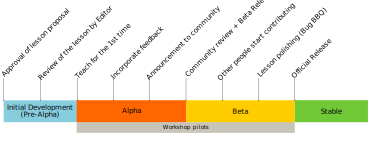
\includegraphics{figures/release_timeline.pdf}
\caption{\label{fig:release-timeline}release timeline}
\end{figure}

Lessons start in the \textbf{pre-alpha} stage - this stage
encompasses everything from the initial lesson idea
through the first time the lesson is taught. This
first draft is usually written by an individual
or a small group of people. From this first draft, the
original authors organize an \textbf{alpha pilot} workshop at
their home organisation, and collect and incorporate
feedback from learners and co-instructors. They go
through this iterative process a few times to bring the
lesson to where it is ready to be taught by other
members of The Carpentries community.

When it is ready for broader teaching and contributions,
the lesson is published for
the first time on Zenodo and is now in the \textbf{beta}
stage. The Carpentries staff will assist the lesson
authors in organising \textbf{beta pilots}.
\textbf{Beta pilots}
should be hosted at a different organisation, and
ideally in a different country than the alpha pilots.
There are generally two or three beta pilots over a
period of six months.

After beta pilots, the lesson authors and Maintainers
incorporate feedback and produce a polished version of
the lesson. It is now mature enough and
documented enough so that anyone interested can teach it. The lesson is published on \href{https://zenodo.org/communities/carpentries/?page=1\&size=20}{Zenodo} and listed on the
Lessons page for the appropriate
Lesson Program. It is added to The Carpentries
\href{http://carpentries.org/request-workshop}{workshop request form}, and becomes an officially
supported lesson. The lesson is now considered \textbf{stable} and will remain in this stage for as long
as it has active support from its Maintainer team.

Lessons with grant support may be eligible for
support from The Carpentries staff in some or all of
these stages. If you are pursuing grant funding for
lesson development, please get in touch with us at
\href{mailto:team@carpentries.org}{\nolinkurl{team@carpentries.org}} to discuss opportunities for staff
support.

\hypertarget{where-to-start}{%
\section{Where to start}\label{where-to-start}}

Before you start developing a new lesson, check
to see if there are already people working on creating
a lesson for this topic. The \href{https://github.com/carpentries-incubator/proposals/blob/master/README.md}{Carpentries Incubator} is where our community comes
together to talk about lesson ideas and find
collaborators. You can check existing \href{https://github.com/carpentries-incubator/proposals/issues}{issues}
or start a new issue if you don't see any discussions
on your topic. The \href{https://github.com/carpentries-incubator/proposals/blob/master/ISSUE_TEMPLATE.md}{issue template} has
a short set of questions for you to answer. Your answers
to these questions will help us to determine an
appropriate next step for your lesson materials or
idea. It's a good idea to also post to our
\href{https://carpentries.topicbox.com/groups/discuss}{discussion forum} and general \href{https://swc-slack-invite.herokuapp.com/}{Slack channel} to point interested people to your
Incubator issue.

Once you've submitted an issue to The Incubator,
you will be directed towards one of the following
tracks:

\begin{enumerate}
\def\labelenumi{\arabic{enumi}.}
\tightlist
\item
  the Official Track
\item
  the Community Track
\item
  the Carpentries Lab Track
\end{enumerate}

\begin{figure}
\centering
\includegraphics{figures/lesson-development-tracks.png}
\caption{Lesson development tracks}
\end{figure}

\hypertarget{official-track}{%
\subsection{Official Track}\label{official-track}}

If The Carpentries have committed to develop a lesson
on this topic (usually through grant funding), our
Curriculum Team will work closely with you from
pre-alpha through stable release, providing support on
each step of the process. Your lesson will be
developed in one of the official Lesson Program GitHub
organisations.

\hypertarget{community-track}{%
\subsection{Community Track}\label{community-track}}

If The Carpentries has not committed to develop a
lesson on this topic, but the lesson is potentially of
general interest to our community, the lesson authors
will complete the development process independently.
You will develop
your lesson in the Carpentries Incubator and it will be
made available through the Incubator
website. If the lesson attracts a strong community
of contributors, it will be considered for adoption
as an official Carpentries lesson.

\hypertarget{carpentries-lab-track}{%
\subsection{Carpentries Lab Track}\label{carpentries-lab-track}}

This track is available for lessons on the Community
Track that do not attract a strong contributor
community. Lesson authors will be able to submit their
materials for peer-review. After the peer-review
process, the lessons will be hosted in The Carpentries
Lab and will be officially endorsed by The Carpentries
as high-quality resources.

\hypertarget{early-development-pre-alpha-through-alpha}{%
\section{Early development (pre-alpha through alpha)}\label{early-development-pre-alpha-through-alpha}}

We will create a repository for you in the appropriate
GitHub organization, using our
\href{https://github.com/carpentries/styles}{lesson template}. You will use the
guidelines in the first five chapters of this handbook
to develop your content. The Curriculum Team will
be available to answer questions about the template
and provide pedagogical guidance. For lessons on the
Official Track, authors will meet regularly with
a member of the Curriculum Team to work through the
lesson drafting process.

\hypertarget{field-testing-alpha-stage}{%
\section{Field testing: alpha stage}\label{field-testing-alpha-stage}}

Once your lesson is ready to be taught for the first
time, it will enter the \textbf{alpha stage}. Field-testing a
lesson is a good opportunity to receive and incorporate
feedback from learners, instructors, and workshop
helpers who can compare their expectations to
reality. The initial feedback gathered during these first
workshops is really important.

During alpha pilot workshops, instructors and helpers should take detailed notes, including:\\
- amount of time used to teach each section\\
- amount of time used for each exercise\\
- technical issues that arose during installation\\
- bugs or parts of the lesson code that didn't work as expected\\
- incorrect or missing exercise solutions\\
- questions learners asked (and their answers)\\
- parts of the lesson that were confusing for learners

These notes can be collected in an Etherpad, Google Doc, or other collaborative document that is shared
with co-instructors and workshop helpers. This document should not be shared with workshop learners,
as it would add significantly to their cognitive load.

After the workshop, instructors should share the notes document with the lesson authors - who
will convert the notes into individual issues in the lesson repo. For two-day workshops, lesson authors should expect
to spend at least four hours to create follow-up issues, and at least
eight hours to putting in PRs to fix these issues. For two pilot workshops, this translates
to \textasciitilde{}24 hours of work, which can be distributed among the lesson authors.

After incorporating workshop feedback, the lesson is
now ready to be published. For lessons on the Official
Track, our Curriculum Team will create a publication
record on \href{https://zenodo.org/communities/carpentries/?page=1\&size=20}{Zenodo}. Lesson authors on the Community or CarpentriesLab tracks
may also choose to publish their lesson on Zenodo. At this stage, the lesson is in \textbf{beta}.

\hypertarget{polishing-beta-stage}{%
\section{Polishing: beta stage}\label{polishing-beta-stage}}

Now that the lesson has been published, it is ready
for teaching by instructors outside of the original
authorship team, and for contributions from the broader
Carpentries community. For lessons on the Official Track,
Carpentries staff will assist lesson authors in recruiting instructors
to teach beta pilots. Authors for non-Official Track lessons
can recruit beta pilot hosts and instructors through our
\href{https://carpentries.topicbox.com/groups/discuss}{discussion list}, \href{https://swc-slack-invite.herokuapp.com/}{Slack organization},
on Twitter, and through domain-specific mailing lists
or other community groups they are part of.
For more information about the role played by
and qualifications needed to be a beta pilot instructors, see
our chapter on \href{https://cdh.carpentries.org/community-development-roles.html\#beta-pilot-instructors}{community development roles}.

The \textbf{beta stage} lasts approximately 6 months. During this time, members of
The Carpentries community can teach it and contribute to the content of the lesson.
The main goal of this phase of the lesson development is to develop the documentation
needed to ensure that people who have not contributed to the initial development
efforts of the lesson have enough information to teach it effectively.

Beta pilot instructors and helpers should take notes similar
to those described above for alpha pilots, but should (hopefully!)
notice fewer bugs and other issues. As with alpha pilots,
beta pilot instructors will provide the lesson authors with
the notes they've collected during the workshop and the authors
will convert those notes to issues and PRs to resolve concerns
raised during the workshop. Maintainers and other community members
will be involved with this clean-up phase as well.

After this polishing process, and a final check by a member of the
Curriculum Team, your lesson will be published again on Zenodo,
this time in its \textbf{stable state}. Official Track lessons will be added to
the appropriate Lesson Program lessons page (e.g. \href{https://datacarpentry.org/lessons/}{Data Carpentry's lessons page})
and to our \href{http://carpentries.org/request-workshop}{workshop request form}. Anyone may now request a centrally-organized
Carpentries workshop using this curriculum.

For lessons on the CarpentriesLab track, authors will submit their stable stage lessons for review.
The CarpentriesLab Editor will select 2-3 reviewers within The Carpentries community with teaching experience and/o
r appropriate domain expertise, who will provide an open and friendly review of the lesson.
After incorporating feedback and comments from the reviewers, your lesson will be badged
``Reviewed by the Carpentries Community'' and will be listed on our websites as such. During this process,
you will have the possibility to include a short paper describing your
lesson in the GitHub repository and have your lesson considered for publication in
\href{http://jose.theoj.org/}{JOSE}, the Journal of Open Science Education.
\textbf{This review process is in development and we are not yet accepting submissions. Please watch for
announcements as we roll out this program.}

\hypertarget{the-stable-lesson-maintenance-and-lesson-releases}{%
\section{The stable lesson: Maintenance and lesson releases}\label{the-stable-lesson-maintenance-and-lesson-releases}}

Congratulations! Your lesson has now been published and is being actively taught by the community.
That means you're done, right? Not exactly. In order to ensure that your wonderful lesson materials
continue to be relevant and useful, you'll need to build and train a team of lesson Maintainers, who
are responsible for day-to-day upkeep and periodic publication of the lesson.

In a \href{community-development-roles\#lesson-maintainers}{previous chapter}, we discussed the process for recruiting and training Maintainers. Here, we
will focus on the responsibilities of Maintainers, their day-to-day workflow, and their involvement
in the lesson release process.

As your lesson is taught, workshop instructors and helpers will post issues and pull requests to
the lesson's GitHub repository. These will range from typo corrections, to installation problems,
to recommendations for changing the libraries or function calls demonstrated in the lesson, and will
therefore require different levels of consideration and technical expertise to implement. A typo
correction will probably be taken care of independently by a single Maintainer,
while a proposal to change
the plotting system used in the lesson from matplotlib to seaborn will require significant
discussion. Each lesson Maintainer team will develop their own strategies for managing their work,
but we recommend the following as a starting point.

\begin{itemize}
\tightlist
\item
  Maintainers for a lesson should set a regular meeting to discuss any unresolved issues that have arisen and to decide on the division of responsibilities until
  their next meeting.\\
\item
  One Maintainer commits to monitor the repo daily and respond to new issues and PRs to acknowledge them,
  thank the contributor, and apply appropriate \href{https://docs.carpentries.org/topic_folders/maintainers/github_labels.html}{issue tags}.\\
\item
  Once a week, one Maintainer looks at the list of active issues and PRs and assigns each to one team member, based on the time commitment and availability discussed at that month's meeting.\\
\item
  Individual team members work on resolving issues and PRs, as assigned, asking
  their co-Maintainers for review when needed.
\end{itemize}

\textbf{The Maintainer community is working on developing a set of guidelines and template
language for responding to common situations. These guidelines will be added
to this section when they become available.}

The above description focuses on Maintainers' ongoing duties. Maintainers are
also involved with lesson releases, which take place roughly every six months.
Information about lesson releases will be added to a future version of this
handbook.

\hypertarget{technological-introductions}{%
\chapter{Technological introductions}\label{technological-introductions}}

Our goal is to make
developing and contributing to lessons as simple and accessible
as possible. The more people who are able to contribute to a
lesson, the more we can harness community knowledge and
experience to create materials that are teachable and applicable
in a range of learning contexts. We recognize that technology
can be a major barrier to contribution, and we are currently
working on a major update to our lesson infrastructure to reduce
this barrier. This chapter reflects our current lesson
infrastructure and describes what lesson authors and other
contributors need to know to use The Carpentries lesson template.
In the individual sections below, we have noted whether particular
technological knowledge will remain necessary or be phased out
in upcoming infrastructure updates.

What knowledge are we assuming lesson authors will have?
What knowledge will this chapter help them gain?

\hypertarget{lesson-hosting-and-rendering}{%
\section{Lesson hosting and rendering}\label{lesson-hosting-and-rendering}}

The Carpentries hosts all of our lessons on \href{https://github.com}{GitHub}. We use a
shared \href{http://carpentries.github.io/lesson-example/setup.html}{lesson template} to provide aesthetic and structural
consistency across our lessons. Template files for each lesson are
rendered into a webpage using \href{https://jekyllrb.com/}{Jekyll} -
a static site generator which is written in \href{https://www.ruby-lang.org/en/}{Ruby}.

You do \emph{not} need to know Ruby or Jekyll to write
or contribute to a Carpentries lesson. However, you will need to
have these software packages installed on your computer if you
want to view your lesson materials locally before pushing them
to GitHub.

Information about installing Ruby and Jekyll is available in the APPENDIX.

\hypertarget{using-the-lesson-template}{%
\section{Using the lesson template}\label{using-the-lesson-template}}

Each lesson is made up of \emph{episodes}, which are focused on a
particular topic and
include time for both teaching and exercises. A lesson repository
(or ``repo'') includes one file for each episode,
and a set of helper files that are required to build
the lesson webpage. Most of these helper files are standardized
across all of our lessons and aren't something that lesson
authors or contributors need to interact with. In this section,
we will focus only on the files that you are likely to
interact with. If you're interested in the details
of how the template is structured, and what each of the files
does, these details are provided in APPENDIX. We recommend not
spending time learning these details now, as we are in the
process of greatly simplifying our lesson template.

\hypertarget{creating-your-lesson-repository}{%
\subsection{Creating your lesson repository}\label{creating-your-lesson-repository}}

The following sections will guide you through the pieces of
the lesson template that you will need to modify to create your lesson.
In order to follow along with these examples, you can start by creating your
lesson repository in GitHub. To do this, follow \href{http://carpentries.github.io/lesson-example/setup.html}{the setup instructions
on our example lesson}.

\hypertarget{lesson-homepage}{%
\subsection{Lesson homepage}\label{lesson-homepage}}

The lesson homepage provides an overview of the lesson, including
any prequisites, an introduction to the
dataset used, a schedule showing
the episodes and the time alloted for each, and any other
information learners will need for the lesson.

For inspiration to guide you in writing your lesson homepage,
check out these examples for \href{https://datacarpentry.org/python-ecology-lesson/}{Data Carpentry}, \href{http://swcarpentry.github.io/git-novice/}{Software Carpentry}, and \href{https://librarycarpentry.org/lc-open-refine/}{Library Carpentry}.

The lesson homepage is built from the \texttt{index.md} file, which is
automatically created when you initialize a lesson repository. You
will need to add the following to this file:

\begin{enumerate}
\def\labelenumi{\arabic{enumi}.}
\tightlist
\item
  A few paragraphs of explanatory text describing the lesson.
\item
  One or more \texttt{.prereq} boxes detailing the lesson's prerequisites, giving an overview of the dataset, and/or calling attention to the lesson's Instructor notes.
\end{enumerate}

The schedule will automatically be included in the lesson homepage based on information present in the
episode files.

\hypertarget{episode-files}{%
\subsection{Episode files}\label{episode-files}}

The majority of a lessons content is in its episode files.
Episode files are stored in the \texttt{\_episodes/} folder within your lesson repo (or in \texttt{\_episodes\_rmd/} for lessons written in R).
Episode file names must start with a two-digit identifier number (e.g. \texttt{01}) followed
by a short descriptive name, separated by a dash (\texttt{-}). For example \texttt{02-loop.md}, \texttt{03-lists.md}.
The numeric identifier is used to place your episode files in the correct sequence within the lesson.
Episode files are written in \emph{Markdown} (more on that in a moment) or \emph{RMarkdown}.

\hypertarget{episode-headers}{%
\subsubsection{Episode headers}\label{episode-headers}}

When your lesson repository is created, it will start out with one pre-made episode file (\texttt{01-introduction.md}).
You can use this file as a template for creating each of your episode files, as it provides an
example of how these files must be structured. The content of this pre-made episode file is shown below:

\begin{verbatim}
---
title: "Introduction"
teaching: 0
exercises: 0
questions:
- "Key question (FIXME)"
objectives:
- "First learning objective. (FIXME)"
keypoints:
- "First key point. Brief Answer to questions. (FIXME)"
---
FIXME


\end{verbatim}

The material between the first and second instances of \texttt{-\/-\/-} is called the \emph{YAML header}. The information
stored in the YAML header is used by the lesson template to populate important parts of the lesson webpage.
This section explains each component of the YAML header and what that information is used for.

For each episode, you will need to create a copy of this file and:

\begin{enumerate}
\def\labelenumi{\arabic{enumi}.}
\tightlist
\item
  Replace \texttt{Introduction} with the episode title (\textbf{not} the lesson title) in quotation marks. The episode
  title will appear on the episode page and in the schedule that appears on the lesson homepage.
\item
  Enter an estimated number of minutes for teaching the episode and an estimated number of minutes for learners to spend completing challenge problems (including class discussion of challenge solutions). These time estimates
  will likely be updated by Instructors as they get real-world data on how learners respond to the pacing of
  the episodes, but it is useful to have a starting point to benchmark from. The lesson template creates a schedule
  from these time estimates and places it on the lesson homepage.
\item
  Replace \texttt{Key\ question\ (FIXME)} with 1-3 motivating questions for the episode, each on a new line and in quotation marks. These motivating questions will appear in the schedule on the lesson homepage.
\item
  Replace \texttt{First\ learning\ objective.\ (FIXME)} with 3-7 learning objectives for the episode, each on a new line and in quotation marks. For information on writing useful learning objectives, see the \href{https://carpentries.github.io/curriculum-development/developing-content.html}{Developing Content} chapter.
\item
  Replace \texttt{First\ key\ point.\ Brief\ Answer\ to\ questions.\ (FIXME)} with 3-7 major take-aways from the episode. For
  information on how to distill an episode's key points, see the \href{https://carpentries.github.io/curriculum-development/developing-content.html}{Developing Content} chapter. Key points for all episodes are shown
  together in the lesson's reference page.
\end{enumerate}

\hypertarget{episode-content}{%
\subsubsection{Episode content}\label{episode-content}}

After the YAML header, your episode file will contain the content for that episode. This content will likely
include:

\begin{itemize}
\tightlist
\item
  paragraphs of text
\item
  lists
\item
  tables
\item
  images or figures
\item
  code chunks
\item
  special blockquotes, including exercises and solutions (described below)
\end{itemize}

This content will be written in \emph{Markdown}, a light-weight markup language that makes it possible to create
fancy HTML pages using only a few formating tricks. In this section, we'll cover only the Markdown syntax that
you will need in order to create the content types listed above. You can find more information about Markdown
at \url{https://commonmark.org/help/}.

\begin{enumerate}
\def\labelenumi{\arabic{enumi}.}
\tightlist
\item
  Paragraphs of text - To create text paragraphs in Markdown, just type as you normally would! A few neat tricks:
\end{enumerate}

\begin{itemize}
\tightlist
\item
  surround text with a single pair of stars (\texttt{*}) to make text \emph{italic} (\texttt{*italic*})
\item
  use a double pair of stars to make text \textbf{bold} (\texttt{**bold**})
\item
  create headers by starting a line of text with two hash signs (\texttt{\#\#})
  There are lots of other fancy things you can do, but this should get you started!
\end{itemize}

\begin{enumerate}
\def\labelenumi{\arabic{enumi}.}
\tightlist
\item
  Lists - To create a numbered list in Markdown, do this:
\end{enumerate}

\begin{verbatim}
1. A
1. numbered
1. list
\end{verbatim}

This will show up like this:

\begin{enumerate}
\def\labelenumi{\arabic{enumi}.}
\tightlist
\item
  A
\item
  numbered
\item
  list
\end{enumerate}

Hint: You can use sequential numbers if you want, but it's easier to update the list later if you use only 1s.
Markdown will create the sequence for you.

To create an un-numbered list in Markdown, do this:

\begin{verbatim}
* An
* unnumbered
* list
\end{verbatim}

This will show up like this:

\begin{itemize}
\tightlist
\item
  An
\item
  unnumbered
\item
  list
\end{itemize}

\begin{enumerate}
\def\labelenumi{\arabic{enumi}.}
\tightlist
\item
  Tables - To insert a small table into your episode, do this:
\end{enumerate}

\begin{verbatim}
| Category | Item | 
|--------- | ---- |
| Food     | Sandwich |
| Drink    | Tea | 
| Food     | Apple |
\end{verbatim}

This will show up like this:

\begin{longtable}[]{@{}ll@{}}
\toprule
Category & Item\tabularnewline
\midrule
\endhead
Food & Sandwich\tabularnewline
Drink & Tea\tabularnewline
Food & Apple\tabularnewline
\bottomrule
\end{longtable}

\begin{enumerate}
\def\labelenumi{\arabic{enumi}.}
\tightlist
\item
  Images or figures - Place a copy of the image you would like to display into the \texttt{fig} directory. You can
  then link to the figure using the syntax:
\end{enumerate}

\begin{verbatim}
![Figure Description](../fig/figure_file_name.svg)
\end{verbatim}

Note about alt text. Question: Is this the ``proper'' way to insert a figure link?

\begin{enumerate}
\def\labelenumi{\arabic{enumi}.}
\tightlist
\item
  Code chunks - As discussed in \href{https://carpentries.github.io/curriculum-development/developing-content.html}{an earlier chapter}, Carpentries workshops are taught using participatory
  live coding. Instructors
  type the code as they teach it and learners type along with the Instructor. For more information about how
  live coding works, and what its advantages and disadvantages are, read that section of our
  \href{https://carpentries.github.io/instructor-training/14-live/index.html}{Instructor Training program}. The fact
  that Carpentries workshops are taught using live coding means that much of your episode content will be
  \emph{code chunks} - short blocks of code that learners type along with the Instructor and evaluate on their own
  machines. Each code chunk should correspond to one interactive session. If learners will be
  running the code as two distinct commands, that code should be displayed as two distinct chunks in the episode
  file.
\end{enumerate}

You can add a code chunk to your episode using the following syntax:

\begin{verbatim}
~~~
pwd
~~~
{: .source}
\end{verbatim}

Which will show up like:

\begin{Shaded}
\begin{Highlighting}[]
\BuiltInTok{pwd}
\end{Highlighting}
\end{Shaded}

Code chunks that learners should type out with the Instructor should use the \texttt{\{:\ .source\}} tag as shown above.
Chunks that show expected output should use the \texttt{\{:\ .output\}} tag. Chunks that show an expected error
message should use the \texttt{\{:\ .error\}} tag.

The generic \texttt{\{:\ .source\}} tag can be used for all programming languages. To make your code more stylish,
you can use a language-specific tag (instead of \texttt{\{:\ .source\}}). This will add things like syntax highlighting
to your code. The language-specific tags available with our lesson template are:

\begin{itemize}
\tightlist
\item
  \texttt{\{:\ .language-bash\}}
\item
  \texttt{\{:\ .html\}}
\item
  \texttt{\{:\ .language-make\}}
\item
  \texttt{\{:\ .language-matlab\}}
\item
  \texttt{\{:\ .language-python\}}
\item
  \texttt{\{:\ .language-r\}}
\item
  \texttt{\{:\ .language-sql\}}
\end{itemize}

You don't need to use these language-specific tags, but they make your lesson a little prettier.

\begin{enumerate}
\def\labelenumi{\arabic{enumi}.}
\tightlist
\item
  Special blockquotes - Exercises, solutions, helpful tips, and a few other types of special information are
  formatted as blockquotes within the episode file. Each blockquote has the same general structure, but ends
  with a different tag. The ending tag determines how the blockquote will appear on the lesson webpage. The
  general structure of a blockquote is:
\end{enumerate}

\begin{verbatim}
> ## Title
>
> text
> text
> text
{: .callout}
\end{verbatim}

where the \texttt{\{:\ .callout\}} tag should be replaced with one of the following as appropriate:

\begin{itemize}
\tightlist
\item
  \texttt{\{:\ .callout\}} for sharing an aside or comment. Use sparingly.
\item
  \texttt{\{:\ .challenge\}} for an exercise.
\item
  \texttt{\{:\ .discussion\}} for a discussion question.
\item
  \texttt{\{:\ .solution\}} for an exercise solution.
\end{itemize}

Additional blockquote tags included in our lesson template are described in APPENDIX, however, the four listed
above should cover all normal use cases for a lesson author.

Exercise solutions are nested within the blockquote for that exercise, as shown below:

\begin{verbatim}
> ## Challenge Title
>
> This is the body of the challenge.
>
> > ## Solution
> >
> > This is the body of the solution.
> {: .solution}
{: .challenge}
\end{verbatim}

Code chunks may also be nested within blockquotes as needed.

\hypertarget{extras}{%
\subsection{Extras}\label{extras}}

So far we've covered how to create and format the content of your lesson homepage (in the \texttt{index.md} file)
and your lesson episodes (in multiple \texttt{.md} files within the \texttt{\_episodes} directory). This covers most of the
files you will need to work with when you create a new lesson. There are a few remaining files that you will
need to populate in order for your lesson to be fully fleshed out and ready to teach:

\begin{enumerate}
\def\labelenumi{\arabic{enumi}.}
\item
  The Reference page (\texttt{reference.md}) - this file will be created automatically and will include a list
  of all of the keypoints that you defined in your episode YAML headers. You don't need to do anything to create
  this list! However, it's a good idea to add a glossary of terms that are used in your lesson.
\item
  The Setup page (\texttt{setup.md}) - this file will be created automatically, but needs to be populated with
  installation instructions for software learners will need to have before begining the lesson. If learners are
  expected to download data prior to the workshop, that data should also be linked and described here. The setup
  page may be \href{http://swcarpentry.github.io/git-novice/setup.html}{quite simple} or
  \href{https://datacarpentry.org/geospatial-workshop/setup.html}{more complex}, but should
  always include installation information for all three major platforms (Windows, Unix/MacOS, Linux).
\item
  The Instructors' Guide (\texttt{\_extras/guide.md}) - this file should provide additional discussion useful to
  instructors,
  but not appropriate for inclusion in the main lessons. Remember not to overload on details, and to keep the
  information here positive and useful for instructors! This guide should include the following sections:
\end{enumerate}

\begin{itemize}
\item
  Lesson motivation and learning objectives - These concepts should be highlighted in the main lesson material,
  but ideas for
  explaining these concepts further can be placed here.
\item
  Lesson design - Most lessons contain more material than can be taught in a single workshop.
  Describe a general narrative (with time estimates) for teaching either a half day
  or full day with this lesson material. You may also choose to include multiple
  options for lesson design, or what material can be skipped while teaching.
  This section may also include recommendations for how this lesson fits into
  the overall workshop.
\item
  Technical tips and tricks - Provide information on setting up your environment for learners to view your
  live coding (increasing text size, changing text color, etc), as well as
  general recommendations for working with coding tools to best suit the
  learning environment.
\item
  Common problems - This can include answers to common learner questions, as well as links to
  resources (blog posts, stack overflow answers, etc) that may solve problems that
  may occur during a workshop.
\end{itemize}

\hypertarget{other-information}{%
\subsection{Other information}\label{other-information}}

In addition to populating the lesson homepage, lesson content (episodes),
Instructors' guide, and other lesson-specific
pages, lesson authors need to make a few changes to the template
files to make sure that the lesson has all of the neccessary
information.

\begin{enumerate}
\def\labelenumi{\arabic{enumi}.}
\tightlist
\item
  In the \texttt{\_config.yml} file,
\end{enumerate}

\begin{itemize}
\tightlist
\item
  set the \texttt{carpentry} variable to the appropriate lesson program,
\item
  set \texttt{title} to be the overall title for your lesson,
\item
  set \texttt{email} to the correct contact email for your lesson.
\end{itemize}

\begin{enumerate}
\def\labelenumi{\arabic{enumi}.}
\item
  In the \texttt{CONTRIBUTING.md} file, change the \texttt{issues} and \texttt{repo} links to match the URLs of your lesson.
\item
  In the \texttt{CITATION} file, add information about how to cite your lesson.
\item
  The \texttt{AUTHORS} file should include a list of the lesson's authors.
\end{enumerate}

\hypertarget{special-notes-on-rmarkdown}{%
\subsection{Special notes on RMarkdown}\label{special-notes-on-rmarkdown}}

Coming soon!

\hypertarget{working-on-github}{%
\section{Working on GitHub}\label{working-on-github}}

GitHub is a web-based service for hosting code under version control. In addition to being a technical
platform, GitHub is also a social media platform and has its own standards around etiquite and interaction. This
section describes how The Carpentries community tends to interact on GitHub and gives you some tips for
navigating this new social scene.

All Carpentries lesson materials, whether they are established or in early development, are hosted publically
on GitHub in one of several \emph{organisations}. The following high-level organisations are managed by The Carpentries:

\begin{itemize}
\tightlist
\item
  \href{https://github.com/carpentries}{carpentries} - hosts The Carpentries website and materials for programs that span individual lesson programs, such as our Instructor Training curriculum and The Carpentries Handbook
\item
  \href{https://github.com/datacarpentry}{datacarpentry} - hosts Data Carpentry specific lesson materials and website
\item
  \href{https://github.com/librarycarpentry}{librarycarpentry} - hosts Library Carpentry specific lesson materials and website
\item
  \href{https://github.com/swcarpentry}{swcarpentry} - hosts Software Carpentry specific lesson materials and website
\item
  \href{https://github.com/data-lessons}{data-lessons} - hosts lessons in development which are targeted to become part of the official Carpentries lesson stack
\item
  \href{http://github.com/carpentrieslab}{carpentrieslab} - community-developed lessons which may or may not become part of the official Carpentries lesson stack
\end{itemize}

In order to contribute to lesson materials, you will need a GitHub account.

To manage changes, we follow \href{https://guides.github.com/introduction/flow/}{GitHub flow}.
Each lesson has two maintainers who review issues and pull requests or encourage others to do so.
The maintainers are community volunteers and have final say over what gets merged into the lesson.
To use the web interface for contributing to a lesson:

\begin{enumerate}
\def\labelenumi{\arabic{enumi}.}
\tightlist
\item
  Fork the originating repository to your GitHub account.
\item
  Within your version of the forked repository, move to the
  default branch (e.g. \texttt{gh-pages}) and
  create a new branch for each significant change being made.
\item
  Navigate to the file(s) you wish to change within the new branches and make revisions as required.
\item
  Commit all changed files within the appropriate branches.
\item
  Create individual pull requests from each of your changed branches
  to the \texttt{gh-pages} branch within the originating repository.
\item
  If you receive feedback, make changes using your issue-specific branches of the forked
  repository and the pull requests will update automatically.
\item
  Repeat as needed until all feedback has been addressed.
\end{enumerate}

When starting work, please make sure your clone of the originating \texttt{gh-pages} branch is up-to-date
before creating your own revision-specific branch(es) from there.
Additionally, please only work from your newly-created branch(es) and \emph{not}
your clone of the originating \texttt{gh-pages} branch.
Lastly, published copies of all the lessons are available in the \texttt{gh-pages} branch of the originating
repository for reference while revising.

If you choose to contribute via GitHub, you may want to look at
\href{https://egghead.io/series/how-to-contribute-to-an-open-source-project-on-github}{How to Contribute to an Open Source Project on GitHub}.

\bibliography{book.bib}

\end{document}
